\documentclass[10pt,twocolumn,letterpaper]{article}

%%%%%%%%% PAPER TYPE  - PLEASE UPDATE FOR FINAL VERSION
% \usepackage[review]{cvpr}      % To produce the REVIEW version
% \usepackage{cvpr}              % To produce the CAMERA-READY version
\usepackage[pagenumbers]{cvpr} % To force page numbers, e.g. for an arXiv version

% Include other packages here, before hyperref.
\usepackage{graphicx}
\usepackage{amsmath}
\usepackage{amssymb}
\usepackage{booktabs}
\usepackage{multirow}
\usepackage{pifont}
\usepackage{xcolor}
\def\etc{etc.\@\xspace}
\newcommand{\TODO}[1]{\textcolor{red}{#1}}
% \usepackage{CJKutf8}
\usepackage{colortbl}
\newcommand{\cc}{\cellcolor[gray]{0.9}}
\newcommand{\tc}[1]{\textcolor{blue}{#1}}
\usepackage{listings}
\definecolor{codegreen}{rgb}{0,0.6,0}
\definecolor{codegray}{rgb}{0.5,0.5,0.5}
\definecolor{codepurple}{rgb}{0.58,0,0.82}
% \definecolor{backcolour}{rgb}{0.95,0.95,0.92}

\lstdefinestyle{mystyle}{
    % backgroundcolor=\color{backcolour},   
    commentstyle=\color{codegreen},
    keywordstyle=\color{magenta},
    numberstyle=\tiny\color{codegray},
    stringstyle=\color{codepurple},
    % basicstyle=\ttfamily\footnotesize,
    basicstyle=\ttfamily\small,
    breakatwhitespace=false,         
    breaklines=true,                 
    captionpos=b,                    
    keepspaces=true,                 
    numbers=left,                    
    numbersep=5pt,                  
    showspaces=false,                
    showstringspaces=false,
    showtabs=false,                  
    tabsize=2
}
\lstset{style=mystyle}

% \usepackage{cancel}
% \newcommand{\lee}[1]{\textcolor{red}{#1}}
% \newcommand{\jr}[1]{\textcolor{blue}{#1}}

% It is strongly recommended to use hyperref, especially for the review version.
% hyperref with option pagebackref eases the reviewers' job.
% Please disable hyperref *only* if you encounter grave issues, e.g. with the
% file validation for the camera-ready version.
%
% If you comment hyperref and then uncomment it, you should delete
% ReviewTempalte.aux before re-running LaTeX.
% (Or just hit 'q' on the first LaTeX run, let it finish, and you
%  should be clear).
\usepackage[pagebackref,breaklinks,colorlinks]{hyperref}
\usepackage[accsupp]{axessibility}  % Improves PDF readability for those with disabilities.


% Support for easy cross-referencing
\usepackage[capitalize]{cleveref}
\crefname{section}{Sec.}{Secs.}
\Crefname{section}{Section}{Sections}
\Crefname{table}{Table}{Tables}
\crefname{table}{Tab.}{Tabs.}


%%%%%%%%% PAPER ID  - PLEASE UPDATE
\def\cvprPaperID{5440} % *** Enter the CVPR Paper ID here
\def\confName{CVPR}
\def\confYear{2023}


\begin{document}

%%%%%%%%% TITLE - PLEASE UPDATE
\title{Run, Don't Walk: Chasing Higher FLOPS for Faster Neural Networks}
\author{Jierun Chen\textsuperscript{1}, Shiu-hong Kao\textsuperscript{1}, Hao He\textsuperscript{1} \\
Weipeng Zhuo\textsuperscript{1}, Song Wen\textsuperscript{2}, Chul-Ho Lee\textsuperscript{3}, S.-H. Gary Chan\textsuperscript{1}\\
\textsuperscript{1}HKUST,
\textsuperscript{2}Rutgers University,
\textsuperscript{3}Texas State University\\
% {\tt\small \{jcheneh, wzhuo, gchan\}@cse.ust.hk, {hheat, skao}@connect.ust.hk, song.wen@rutgers.edu, chulho.lee@txstate.edu }
}
\maketitle


%%%%%%%%% BODY TEXT
\begin{abstract}
Segment Anything Model 2 (SAM 2) has emerged as a powerful tool for video object segmentation and tracking anything. Key components of SAM 2 that drive the impressive video object segmentation performance include a large multistage image encoder for frame feature extraction and a memory mechanism that stores memory contexts from past frames to help current frame segmentation. The high computation complexity of multistage image encoder and memory module has limited its applications in real-world tasks, e.g., video object segmentation on mobile devices. To address this limitation, we propose EfficientTAMs, lightweight track anything models that produce high-quality results with low latency and model size. Our idea is based on revisiting the plain, nonhierarchical Vision Transformer (ViT) as an image encoder for video object segmentation, and introducing an efficient memory module, which reduces the complexity for both frame feature extraction and memory computation for current frame segmentation. We take vanilla lightweight ViTs and efficient memory module to build EfficientTAMs, and train the models on SA-1B and SA-V datasets for video object segmentation and track anything tasks. We evaluate on multiple video segmentation benchmarks including semi-supervised VOS and promptable video segmentation, and find that our proposed EfficientTAM with vanilla ViT perform comparably to SAM 2 model (HieraB+SAM 2) with $\sim$2x speedup on A100 and $\sim$2.4x  parameter reduction. On segment anything image tasks, our EfficientTAMs also perform favorably over original SAM with $\sim$20x  speedup on A100 and $\sim$20x  parameter reduction. On mobile devices such as iPhone 15 Pro Max, our EfficientTAMs can run at $\sim$10 FPS for performing video object segmentation with reasonable quality, highlighting the capability of small models for on-device video object segmentation applications. 
\end{abstract}
\section{Introduction}
Reinforcement Learning from Human Feedback (RLHF) is a technique that can be used to align an agent --- such as a Large Language Model (LLM) --- to human preferences and lead to more truthful, more helpful, less harmful and more preferred outputs \cite{ouyang2022training}. Proximal Policy Optimization (PPO) \cite{schulman2017proximal} and Direct Preference Optimization (DPO) \cite{rafailov2023direct} are two such aligment techniques which have been extensively used to improve the quality of LLM outputs, leading to instruction following agents or chat assistants which are quickly approaching human-baselines in a variety of knowledge and reasoning tasks \cite{open-llm-leaderboard, clark2018think, zellers2019hellaswag, hendrycks2021measuring, lin2022truthfulqa, DBLP:journals/corr/abs-1907-10641, DBLP:journals/corr/abs-2110-14168}.

However, recent research has shown that RLHF may actually hurt an LLM's reasoning abilities rather than improving it. One study \cite{bekbayev2023poison} discovered that performing alignment during the Supervised Fine-Tuning (SFT) stage of training may lead to worse performance on reasoning benchmarks, and another \cite{bai2022training} discovered that SFT alone outperforms RLHF for smaller models with the benefits of RLHF only emerging for models with more than 1 Billion parameters. Ouyang et al. \cite{ouyang2022training} also reports an increased tendency for RLHF models to make up information in closed domain tasks (``hallucination'') compared to models trained with SFT alone.

To combat the the risk of RLHF compromising the abilities of an LLM in favor of producing preferable outputs we introduce Direct Preference Heads (DPH), a novel feature based approach that optimises a reward score produced by the LLM rather than optimising the logits produced by language modelling head. DPH can be used in combination with (or without) existing alignment techniques to allow language models to self-evaluate outputs sampled at inference time and select the highest scoring candidate.

We evaluate the performance of DPH using an efficient 551M parameter LM on a variety of commonsense reasoning and Natural Language Understanding (NLU) tasks. All code used to train our models is available on \anon{\href{https://github.com/Avelina9X/direct-preference-heads}{GitHub}} and we release our model weights on \anon{\href{https://huggingface.co/collections/Avelina/direct-preference-heads-preprint-6612d8a6fa3843352943fd43}{Hugging Face}}.
\section{Related Work}
\label{sec:related_work}
We briefly review prior works on fast and efficient neural networks and differentiate this work from them.

\medskip\noindent\textbf{CNN.} \enspace
CNNs are the mainstream architecture in the computer vision field, especially when it comes to deployment in practice, where being fast is as important as being accurate. Though there have been numerous studies~\cite{sifre2014rigid,singh2019hetconv,chen2019drop,chollet2017xception,zhang2017interleaved,li2021micronet,he2022tackling,zhuo2022semi} to achieve higher efficiency, the rationale behind them is more or less to perform a low-rank approximation. Specifically, the group convolution~\cite{krizhevsky2012imagenet} and the depthwise separable convolution~\cite{sifre2014rigid} (consisting of depthwise and pointwise convolutions) are probably the most popular ones. They have been widely adopted in mobile/edge-oriented networks, such as MobileNets~\cite{howard2017mobilenets,sandler2018mobilenetv2,howard2019searching},
ShuffleNets~\cite{zhang2018shufflenet,ma2018shufflenet}, GhostNet~\cite{han2020ghostnet},
EfficientNets~\cite{tan2019efficientnet,tan2021efficientnetv2}, TinyNet~\cite{han2020model}, Xception~\cite{chollet2017xception}, CondenseNet~\cite{huang2018condensenet,yang2021condensenet}, TVConv~\cite{chen2022tvconv}, MnasNet\cite{tan2019mnasnet}, and FBNet~\cite{wu2019fbnet}. While they exploit the redundancy in filters to reduce the number of parameters and FLOPs, they suffer from increased memory access when increasing the network width to compensate for the accuracy drop. By contrast, we consider the redundancy in feature maps and propose a partial convolution to reduce FLOPs and memory access \emph{simultaneously}. 

\medskip\noindent\textbf{ViT, MLP, and variants.} \enspace
 There is a growing interest in studying ViT ever since Dosovitskiy \etal~\cite{dosovitskiy2020image} expanded the application scope of transformers~\cite{vaswani2017attention} from machine translation~\cite{vaswani2017attention} or forecasting~\cite{wen2022social} to the computer vision field. Many follow-up works have attempted to improve ViT in terms of training setting~\cite{touvron2021training,touvron2022deit,steiner2021train} and model design~\cite{liu2021swin,liu2022swin,wang2021pyramid,graham2021levit,zhong2022tree}. One notable trend is to pursue a better accuracy-latency trade-off by reducing the complexity of the attention operator~\cite{ali2021xcit,vaswani2021scaling,huang2022lightvit,lu2021soft,tang2022quadtree}, incorporating convolution into ViTs~\cite{dai2021coatnet,chen2022mobile,srinivas2021bottleneck}, or doing both~\cite{cai2022efficientvit,li2022efficientformer,pan2022edgevits,mehta2022separable}. Besides, other studies~\cite{tolstikhin2021mlp,lian2021mlp,chen2021cyclemlp} propose to replace the attention with simple MLP-based operators. However, they often evolve to be CNN-like~\cite{liu2022we}. In this paper, we focus on analyzing the convolution operations, particularly DWConv, due to the following reasons: First, the advantage of attention over convolution is unclear or debatable~\cite{wang2022shift,liu2022convnet}. Second, the attention-based mechanism generally runs slower than its convolutional counterparts and thus  becomes less favorable for the current industry~\cite{mehta2021mobilevit,hu2019local}. Finally, DWConv is still a popular choice in many hybrid models, so it is worth a careful examination.
 
\section{Proposed Approach}
\label{sec: approach}
In this section, we present our method of probabilistic Gaussian superposition for efficient 3D semantic occupancy prediction.
We first review the original 3D semantic Gaussian representation~\cite{huang2024gaussian} and its limitations (Sec.~\ref{subsec: old gaussian}).
We then introduce our probabilistic Gaussian modeling and how we derive geometry and semantics predictions based on the multiplication theorem of probability and Gaussian mixture model (Sec.~\ref{subsec: prob modeling}).
Finally, we detail the distribution-based initialization module to effectively initialize probabilistic Gaussians around the occupied area (Sec.~\ref{subsec: initialization}).


\subsection{3D Semantic Gaussian Representation}
\label{subsec: old gaussian}
Vision-centric 3D semantic occupancy prediction~\cite{cao2022monoscene,huang2023tri} aims to obtain the fine-grained geometry and semantics of the 3D scene.
To formulate, the target is to predict voxel-level semantic segmentation result $\mathbf{O}\in \mathcal{C}^{X\times Y\times Z}$ given input images $\mathcal{I}=\{\mathbf{I}_i\}_{i=1}^{N}$, where $\mathcal{C}$, $\{X, Y, Z\}$, $N$ represent the set of predefined classes, the spatial resolution of occupancy and the number of input views, respectively.

To achieve this, 3D semantic Gaussian representation employs a set of $P$ Gaussian primitives $\mathcal{G}=\{\mathbf{G}_i\}_{i=1}^{P}$, with each $\mathbf{G}_i$ describing a local region with its mean $\mathbf{m}_i$, scale $\mathbf{s}_i$, rotation $\mathbf{r}_i$, opacity $a_i$ and semantics $\mathbf{c}_i$.
GaussianFormer interprets these primitives as local semantic Gaussian distributions which contribute to the overall occupancy prediction through additive aggregation:
\vspace{-2mm}
\begin{equation}
    \hat{\mathbf{o}}(\mathbf{x}; \mathcal{G})=\sum_{i=1}^{P}\mathbf{g}_i(\mathbf{x}; \mathbf{m}_i,\mathbf{s}_i,\mathbf{r}_i,a_i,\mathbf{c}_i),
    \label{eq: weighted summation}
    \vspace{-2mm}
\end{equation}
where $\mathbf{g}_i(\mathbf{x};\cdot)$ denotes the contribution of the $i$th semantic Gaussian to $\hat{\mathbf{o}}(\mathbf{x}; \mathcal{G})$ which is the overall occupancy prediction at location $\mathbf{x}$.
The contribution $\mathbf{g}$ is further calculated as the corresponding semantic Gaussian distribution evaluated at location $\mathbf{x}$:
\begin{equation}
    \mathbf{g}(\mathbf{x}; \mathbf{G}) = a\cdot{\rm{exp}}\big(-\frac{1}{2}(\mathbf{x}-\mathbf{m})^{\rm T} \mathbf{\Sigma}^{-1} (\mathbf{x}-\mathbf{m})\big)\mathbf{c},
    \label{eq: gaussian dist}
\end{equation}
\begin{equation}
    \mathbf{\Sigma} = \mathbf{R}\mathbf{S}\mathbf{S}^T\mathbf{R}^T, \quad \mathbf{S} = {\rm{diag}}(\mathbf{s}), \quad \mathbf{R} = {\rm{q2r}}(\mathbf{r}),
\end{equation}
where $\mathbf{\Sigma}$, $\mathbf{R}$, $\mathbf{S}$ represent the covariance matrix, the rotation matrix constructed from the quaternion $\mathbf{r}$ with function ${\rm q2r}(\cdot)$, and the diagonal scale matrix from function ${\rm diag}(\cdot)$.

Although the number of Gaussians is reduced compared with the number of dense voxels thanks to the deformable nature of Gaussian distributions as in Eq.~(\ref{eq: gaussian dist}), several limitations still persist in the 3D semantic Gaussian representation.
First of all, it models both the occupied and unoccupied regions in the same way using the semantic property $\mathbf{c}$, resulting in most Gaussians being classified as empty given the huge proportion of empty space in outdoor scenarios.
Secondly, the semantic Gaussian representation encourages Gaussians to overlap, because the aggregation process in Eq.~(\ref{eq: weighted summation}) independently sums up the contribution of each Gaussian, resulting in unbounded occupancy prediction $\hat{\mathbf{o}}$.
For optimization, the model would learn to allocate more Gaussians to describe the same region due to the unbounded nature of $\hat{\mathbf{o}}$, aggravating the overlap between Gaussians.
These limitations stem from the current interpretation of Gaussians and obstruct the efficiency and effectiveness of the 3D semantic Gaussian representation.
Our method approaches Gaussian-based object-centric representation from a probabilistic perspective, serving as a fundamental solution to these issues, as shown by Figure~\ref{fig:motivation}.


\subsection{Probabilistic Gaussian Superposition}
\label{subsec: prob modeling}
We propose the probabilistic Gaussian superposition as an efficient and effective 3D scene representation.
As shown in Figure~\ref{fig:pipeline}, we decompose the 3D modeling target into geometry and semantics predictions, and adopt the multiplication theorem of probability and the Gaussian mixture model to address them from a probabilistic perspective, respectively.

\textbf{Geometry prediction.}
To restrict Gaussians to represent only occupied regions for geometry prediction, we interpret the Gaussian primitives $\mathcal{G}=\{\mathbf{G}_i\}_{i=1}^{P}$ as the probability of their surrounding space being occupied.
To elaborate, we assign a probability value of 100\% at the centers of Gaussians, which decays exponentially with respect to the distance from the centers $\mathbf{m}$:
\begin{equation}
    \alpha(\mathbf{x};\mathbf{G}) = {\rm{exp}}\big(-\frac{1}{2}(\mathbf{x}-\mathbf{m})^{\rm T} \mathbf{\Sigma}^{-1} (\mathbf{x}-\mathbf{m})\big),
    \label{eq: single prob}
\end{equation}
where $\alpha(\mathbf{x};\mathbf{G})$ denotes the probability of the point $\mathbf{x}$ being occupied induced by Gaussian $\mathbf{G}$.
Eq.~(\ref{eq: single prob}) assigns a high probability of occupancy when the point $\mathbf{x}$ is close to the center of Gaussian $\mathbf{G}$, which prevents any Gaussian from describing empty area.
To further derive the overall probability of occupancy, we assume that the probabilities of a point being occupied by different Gaussians are mutually independent, and thus we can aggregate them according to the multiplication theorem of probability:
\vspace{-1mm}
\begin{equation}
    \alpha(\mathbf{x}) = 1 - \prod_{i=1}^{P}\big(1 - \alpha(\mathbf{x};\mathbf{G}_i)\big),
    \label{eq: multi prob}
    \vspace{-1mm}
\end{equation}
where $\alpha(\mathbf{x})$ represents the overall probability of occupancy at point $\mathbf{x}$. 
In addition to achieving object-centric properties, Eq.~(\ref{eq: multi prob}) also avoids unnecessary overlapping between Gaussians because $\alpha(\mathbf{x}) \ge \alpha(\mathbf{x};\mathbf{G}_i)$ holds for any Gaussian $\mathbf{G}_i$.
This implies that point $\mathbf{x}$ would be predicted occupied if it is close enough to any single Gaussian.


\textbf{Semantics prediction.}
In addition to object-centric anti-overlapping geometry modeling, we still need to achieve the same goals for semantics prediction.
We first remove the channel that represents the empty class from the semantic properties $\mathbf{c}$ of Gaussians since it has been accounted for in geometry prediction.
Then we interpret the set of Gaussians $\mathcal{G}$ as a Gaussian mixture model, where semantics prediction could be formulated as calculating the expectation of semantics given the probabilistic Gaussian mixture model.
Specifically, we take the original opacity properties $a$ as the prior distribution of Gaussians, which is $l^1$-normalized.
Furthermore, we adopt the Gaussian probabilistic distribution parameterized by mean $\mathbf{m}$, scale $\mathbf{s}$ and rotation $\mathbf{r}$ as the conditional probability.
Then we normalize the original semantics properties $\mathbf{c}$ with softmax to ensure the boundedness of predicted semantics.
Finally, we calculate the expectation $\mathbf{e}(\mathbf{x};\mathcal{G})$ as:
\vspace{-1mm}
\begin{equation}
\begin{aligned}
    \mathbf{e}(\mathbf{x};\mathcal{G}) &= \sum_{i=1}^{P} p(\mathbf{G}_i|\mathbf{x})\Tilde{\mathbf{c}}_i 
    = \frac{\sum_{i=1}^{P}p(\mathbf{x}|\mathbf{G}_i)a_i\Tilde{\mathbf{c}}_i}{\sum_{j=1}^{P}p(\mathbf{x}|\mathbf{G}_j)a_j},
\end{aligned}
\label{eq: gmm}
\end{equation}
\begin{small}
\begin{equation}
    p(\mathbf{x}|\mathbf{G}_i) = \frac{1}{(2\pi)^{\frac{3}{2}}|\mathbf{\Sigma}|^{\frac{1}{2}}}{\rm{exp}}\big(-\frac{1}{2}(\mathbf{x}-\mathbf{m})^{\rm T} \mathbf{\Sigma}^{-1} (\mathbf{x}-\mathbf{m})\big),
\end{equation}
\end{small}where $p(\mathbf{G}_i|\mathbf{x})$, $p(\mathbf{x}|\mathbf{G}_i)$ and $\Tilde{\mathbf{c}}_i$ denote the posterior probability of point $\mathbf{x}$ belonging to the $i$th Gaussian distribution, the conditional probability of point $\mathbf{x}$ given the $i$th Gaussian distribution, and the softmax-normalized semantic properties, respectively. 
Compared with Eq.~(\ref{eq: weighted summation})(\ref{eq: gaussian dist}), the gaussian mixture model in Eq.~(\ref{eq: gmm}) normalizes the semantic properties and the contributions from different Gaussians, thus preventing unnecessary overlapping between Gaussians and producing normalized class probabilities directly.

Given the geometry and semantics predictions, we take a simple step forward to combine them to generate the final semantic occupancy prediction:
\begin{equation}
    \hat{\mathbf{o}}(\mathbf{x};\mathcal{G}) = [1-\alpha(\mathbf{x}); \alpha(\mathbf{x})\cdot\mathbf{e}(\mathbf{x};\mathcal{G})],
    \label{eq: final occ}
\end{equation}
where we use the geometry probability $\alpha(\mathbf{x})$ to weight the semantic predictions, and directly take $1 - \alpha(\mathbf{x})$ as the probability of the empty class.

\begin{figure}[t]
\centering
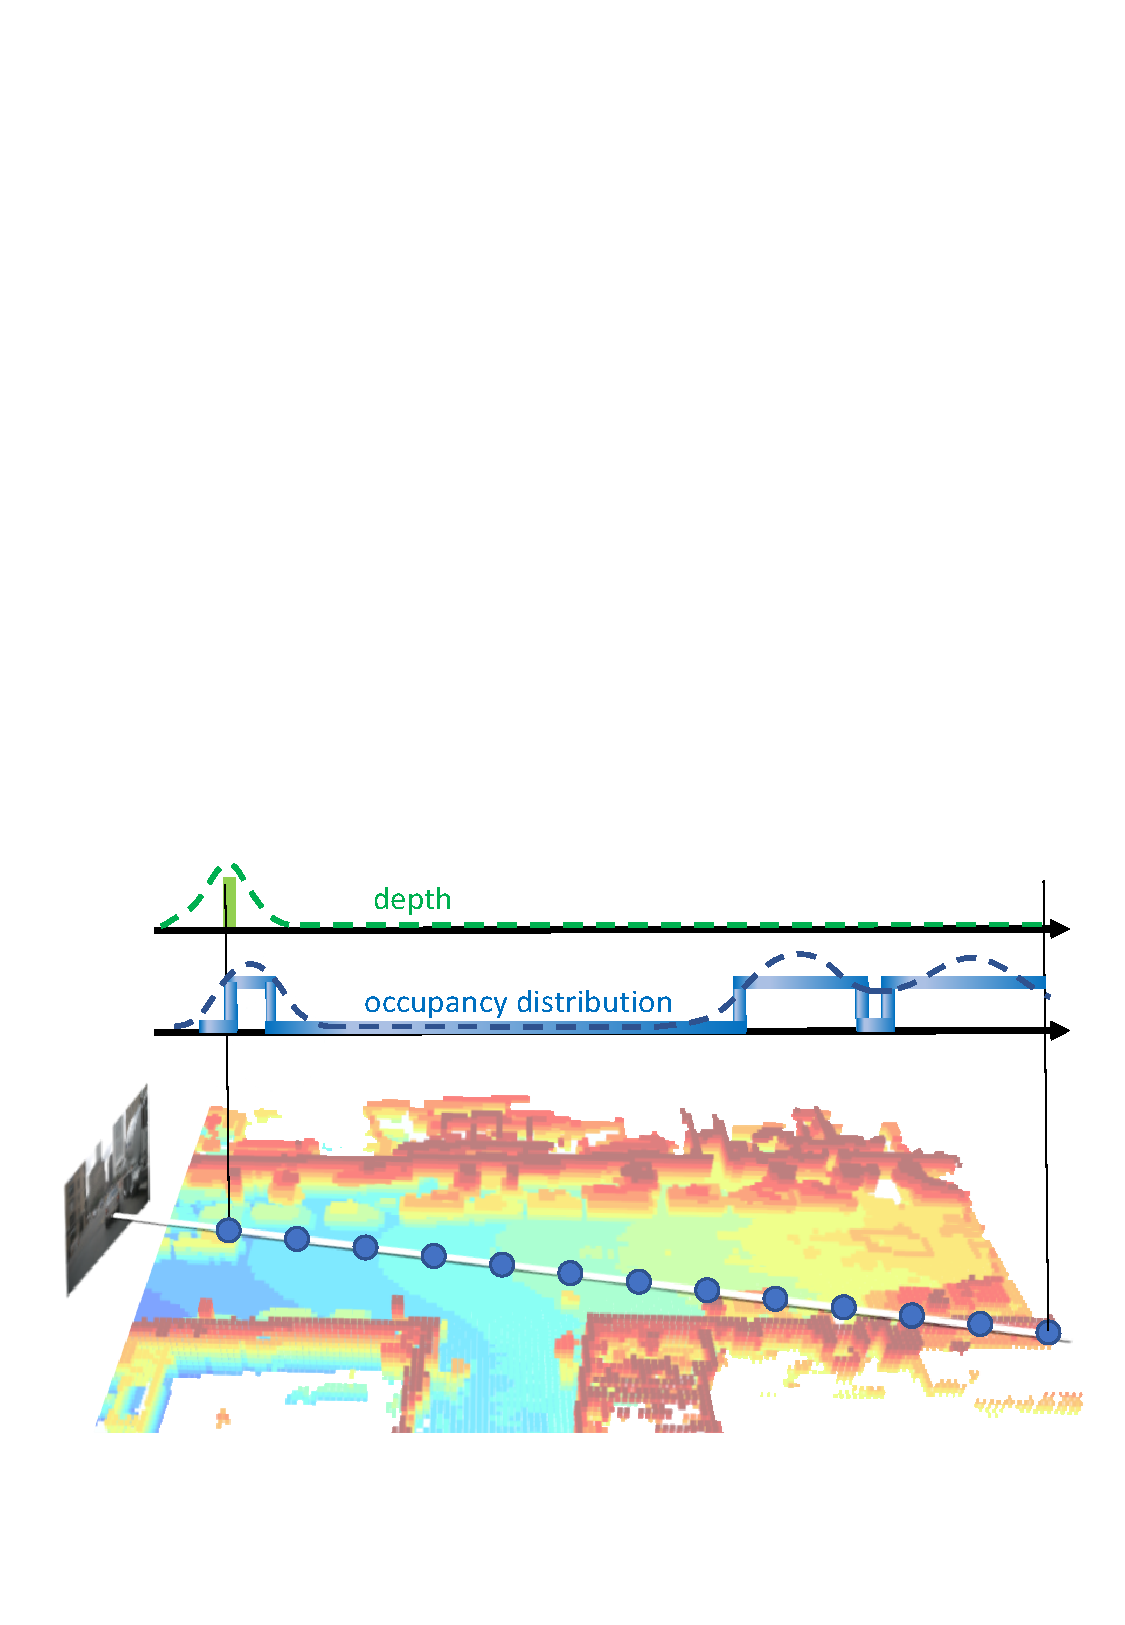
\includegraphics[width=0.95\linewidth]{figures/initialization.pdf}
\vspace{-2mm}
\caption{\textbf{Distribution-based initialization.}
Our initialization scheme learns pixel-aligned occupancy distributions from occupancy annotation, while the depth-based counterpart only captures the surfaces of objects and relies on LiDAR supervision.
}
\label{fig:initialization}
\vspace{-6mm}
\end{figure}

\begin{table*}[t] %
    \caption{\textbf{Surround view 3D semantic occupancy prediction results on nuScenes.} 
    * means supervised by dense occupancy annotations as opposed to original LiDAR segmentation labels.
    Ch. denotes the channel dimension of our model.
    Our method achieves state-of-the-art performance compared with other methods.}
    \small
    \setlength{\tabcolsep}{0.005\linewidth}  
    \vspace{-3mm}  
    \renewcommand\arraystretch{1.05}
    \centering
    \resizebox{\textwidth}{!}{
    \begin{tabular}{l|c c | c c c c c c c c c c c c c c c c}
        \toprule
        Method
        & IoU
        & mIoU
        & \rotatebox{90}{\textcolor{nbarrier}{$\blacksquare$} barrier}
        & \rotatebox{90}{\textcolor{nbicycle}{$\blacksquare$} bicycle}
        & \rotatebox{90}{\textcolor{nbus}{$\blacksquare$} bus}
        & \rotatebox{90}{\textcolor{ncar}{$\blacksquare$} car}
        & \rotatebox{90}{\textcolor{nconstruct}{$\blacksquare$} const. veh.}
        & \rotatebox{90}{\textcolor{nmotor}{$\blacksquare$} motorcycle}
        & \rotatebox{90}{\textcolor{npedestrian}{$\blacksquare$} pedestrian}
        & \rotatebox{90}{\textcolor{ntraffic}{$\blacksquare$} traffic cone}
        & \rotatebox{90}{\textcolor{ntrailer}{$\blacksquare$} trailer}
        & \rotatebox{90}{\textcolor{ntruck}{$\blacksquare$} truck}
        & \rotatebox{90}{\textcolor{ndriveable}{$\blacksquare$} drive. suf.}
        & \rotatebox{90}{\textcolor{nother}{$\blacksquare$} other flat}
        & \rotatebox{90}{\textcolor{nsidewalk}{$\blacksquare$} sidewalk}
        & \rotatebox{90}{\textcolor{nterrain}{$\blacksquare$} terrain}
        & \rotatebox{90}{\textcolor{nmanmade}{$\blacksquare$} manmade}
        & \rotatebox{90}{\textcolor{nvegetation}{$\blacksquare$} vegetation}
        \\
        \midrule
        MonoScene~\cite{cao2022monoscene} & 23.96 & 7.31 & 4.03 &	0.35& 8.00& 8.04&	2.90& 0.28& 1.16&	0.67&	4.01& 4.35&	27.72&	5.20& 15.13&	11.29&	9.03&	14.86 \\
        
        Atlas~\cite{murez2020atlas} & 28.66 & 15.00 & 10.64&	5.68&	19.66& 24.94& 8.90&	8.84&	6.47& 3.28&	10.42&	16.21&	34.86&	15.46&	21.89&	20.95&	11.21&	20.54 \\
        
        BEVFormer~\cite{li2022bevformer} & 30.50 & 16.75 & 14.22 &	6.58 & 23.46 & 28.28& 8.66 &10.77& 6.64& 4.05& 11.20&	17.78 & 37.28 & 18.00 & 22.88 & 22.17 & {13.80} &	\textbf{22.21}\\
        
        TPVFormer~\cite{huang2023tri} & 11.51 & 11.66 & 16.14&	7.17& 22.63	& 17.13 & 8.83 & 11.39 & 10.46 & 8.23&	9.43 & 17.02 & 8.07 & 13.64 & 13.85 & 10.34 & 4.90 & 7.37\\
        
        TPVFormer*~\cite{huang2023tri}  & {30.86} & 17.10 & 15.96&	 5.31& 23.86	& 27.32 & 9.79 & 8.74 & 7.09 & 5.20& 10.97 & 19.22 & {38.87} & {21.25} & {24.26} & {23.15} & 11.73 & 20.81\\

        OccFormer~\cite{zhang2023occformer} & {31.39} & {19.03} & {18.65} & {10.41} & {23.92} & {30.29} & {10.31} & {14.19} & {13.59} & {10.13} & {12.49} & {20.77} & {38.78} & 19.79 & 24.19 & 22.21 & {13.48} & {21.35}\\
        
        SurroundOcc~\cite{wei2023surroundocc} & {31.49} & {20.30}  & {20.59} & {11.68} & {28.06} & \textbf{30.86} & {10.70} & {15.14} & \textbf{14.09} & \textbf{12.06} & \textbf{14.38} & {22.26} & 37.29 & {23.70} & {24.49} & {22.77} & \textbf{14.89} & {21.86}  \\


        GaussianFormer~\cite{huang2024gaussian} & 29.83 & {19.10} & {19.52} & {11.26} & {26.11} & {29.78} & {10.47} & {13.83} & {12.58} & {8.67} & {12.74} & {21.57} & {39.63} & {23.28} & {24.46} & {22.99} & 9.59 & 19.12 \\

        \midrule
        \textbf{Ours} (Ch. = 128) & 30.56 & 20.02 & 20.15 & 12.99 & 27.61 & 30.23 & \textbf{11.19} & 15.31 & 12.64 & 9.63 & 13.31 & 22.26 & 39.68 & 23.47 & 25.62 & 23.20 & 12.25 & 20.73 \\
        
        \textbf{Ours} (Ch. = 192) & \textbf{31.74} & \textbf{20.82} & \textbf{21.39} & \textbf{13.44} & \textbf{28.49} & 30.82 & 10.92 & \textbf{15.84} & 13.55 & 10.53 & 14.04 & \textbf{22.92} & \textbf{40.61} & \textbf{24.36} & \textbf{26.08} & \textbf{24.27} & 13.83 & 21.98  \\
        
        \bottomrule
    \end{tabular}}
    \label{tab: nuscenes results}
    \vspace{-5mm}
\end{table*}


\subsection{Distribution-Based Initialization}
\label{subsec: initialization}
Previous 3D semantic Gaussian representation adopts a learnable initialization strategy, which randomly initializes the properties of Gaussians at the beginning of training, and optimizes this initialization in a data-driven way.
This strategy enables the model to learn a prior distribution of occupancy of the whole dataset, which relies on the subsequent refinement of the network to adapt to the distribution of each individual sample.
However, the local receptive field of Gaussians limits their mobility, which hinders each Gaussian from learning the path to the correct position in subsequent refinement.
And this issue is even more severe for our probabilistic Gaussian superposition where Gaussians are supposed to model only occupied regions.

To remedy this issue, we propose a distribution-based initialization module which provides both more accurate and holistic sample-specific initialization for Gaussians, as shown by Figure~\ref{fig:initialization}.
We supervise the image features from a 2D backbone with the pixel-aligned occupancy distribution derived from the occupancy annotations.
To elaborate, we first determine the origin $\mathbf{b}$ and direction $\mathbf{d}$ of the ray corresponding to each image feature with the camera calibration data.
We then sample $R$ reference points at equal intervals in a fixed depth range along this ray.
For each of these reference points, we query the ground truth occupancy $\mathbf{O}$ at the corresponding location to obtain the binary labels $\mathbf{l}=\{l_i\}_{i=1}^{R}$ indicating whether a reference point is occupied or not.
Then we use $\mathbf{l}=\{l_i\}_{i=1}^{R}$ as supervision to optimize our initialization module, which consists of an image backbone ${\rm B}$ and a distribution predictor ${\rm M}$.
The distribution predictor ${\rm M}$ directly decodes image features into occupancy distributions $\hat{\mathbf{l}}$ along corresponding rays, which are matched against $\mathbf{l}$ using binary cross entropy loss:
\begin{equation}
    loss_{init} = {\rm BCE}\big(\hat{\mathbf{l}}, \mathbf{l}\big) = {\rm BCE}\big({\rm M}({\rm B}(\mathcal{I})), \mathbf{l}\big).
\end{equation}
Different from previous initialization schemes~\cite{li2023voxformer,li2022bevdepth,huang2021bevdet} that predict the depth values with LiDAR supervision, our method learns the holistic occupancy distribution rather than only visible surfaces of the scene, and does not require any additional modality as supervision.

Overall, our distribution-based initialization module initializes the Gaussians, which are subsequently sent into B blocks of attention-based architecture as in GaussianFormer~\cite{huang2024gaussian}. 
Each block consists of self-encoding, image cross-attention, and refinement module, where probabilistic Gaussian properties steadily improve, then the resulting Gaussians are aggregated by our new method that encourages higher utilization of Gaussians.

%
% --- inline annotations
%
\newcommand{\red}[1]{{\color{red}#1}}
\newcommand{\todo}[1]{{\color{red}#1}}
\newcommand{\TODO}[1]{\textbf{\color{red}[TODO: #1]}}
% --- disable by uncommenting  
% \renewcommand{\TODO}[1]{}
% \renewcommand{\todo}[1]{#1}

\usepackage{xcolor}
\usepackage{graphicx}
\usepackage{booktabs}
\usepackage{amsmath} 
\usepackage{amsfonts}
\usepackage{amssymb}
\usepackage{multirow} 
\usepackage{makecell}
\newcommand{\shline}{\Xhline{1.1pt}} % Adjust thickness as desired

\section{Experiments}
\label{sec:experiments}

We present results for supervised video classification and self-supervised masked auto-encoding with frozen representations evaluated on two downstream tasks: video classification and point tracking. To analyse the memory capabilities of our model, we also include a reconstruction task of frames seen in the distant past. Using the same task, we study the generalisation capabilities to longer sequences than seen during training. We follow the ViT scaling configurations and, unless otherwise stated, we use the \textbf{B}ase version for our model for all our experiments. We specify the number of parameters for all models considered in our experiments, and we include in the supplementary material all the training hyperparameters and data augmentations used in all experiments.

\subsection{Supervised video classification}

\par \noindent \textbf{Datasets:}
We use large-scale real-world datasets for the supervised video classification task. Kinetics400~\citep{Carreira_2017_CVPR} contains 241,512 videos\footnote{Kinetics is a dynamic dataset (videos may be removed from
YouTube). Our current version has 241,512 videos, compared to 267,000 videos reported in~\cite{vivit}, so a decrease of almost 10\%, noticeable in the final performance.} across train, validation, and test splits, 10s-long (25fps), spanning 400 classes. This dataset is known to require modelling appearance for successful action recognition. To challenge our model's capability of understanding motion, we also use SSv2 dataset~\citep{goyal2017something}, which contains 220,847 shorter videos (2-6s long), sampled at 12fps, representing 174 classes. This dataset includes actions that differ in finer motion-related details, requiring a deeper temporal understanding, e.g. \textit{pouring something into something} vs \textit{pretending to pour something into something}. 

\par \noindent \textbf{Baselines:}
We use ViViT~\citep{vivit} as our main baseline. We consider the full self-attention version, which patchifies and flattens the entire video, prepends a video class token, then runs self-attention blocks. We also consider the factorised encoder version (ViViT FE), which runs a ViT image model over all the frames, and uses temporal self-attention blocks to integrate the information over time. Finally, we also consider a baseline that uses only LRU recurrent and MLP blocks, configured similar to VideoMamba~\cite{li2024videomambastatespacemodel}, i.e. it does not use self-attention blocks, denoted \textit{PureLRU}. Similar to ViViT, this model first patchifies and flattens the video, prepends a class token, then applies a sequence of recurrent blocks. All baselines use learnt spatio-temporal positional encoding, whereas the proposed \ssm\ uses only spatial positional encoding as the temporal dimension is implicitly modelled through its recurrence.


\par \noindent \textbf{Results:} We include results for training from scratch or using Imagenet pre-trained weights to initialise the weights of the ViT blocks. Figure~\ref{fig:baselines} shows a first comparison between \ssm\ and the above baselines, with all models being trained from scratch on supervised classification on SSv2. We consider the \textbf{S}mall version for all models as the larger \textbf{B}ase version shows stability issues when trained from scratch, as reported in other works as well~\cite{li2024videomambastatespacemodel,vivit}. As expected, the performance on this challenging dataset when training from scratch is far from SOTA, but it clearly shows that the proposed factorisation has superior video modelling capabilities compared to baselines, ViViT-S with full self-attention being the closest competitor. PureLRU's performance is very poor, which is in line with the findings of other works (\eg VideoMamba) who report that bidirectional (non-causal) processing of the input is needed for good performance. 

We report further results comparing against ViViT-B and ViViT-L with full self-attention when using Imagenet pre-trained weights; see Table~\ref{tab:ssv2} for SSv2 results and Table~\ref{tab:kinetics} for Kinetics400 results.
We can observe that our model achieves better performance compared to ViViT baselines on SSv2, but it is slightly below ViViT-L on Kinetics400. This result could reflect the difference between the two datasets mentioned above: outperforming ViViT-L on SSv2 suggests that \ssm\ is superior at modelling motion compared to ViViT, but on Kinetics where the appearance is enough for successful classification, both models are on par. We consider this to be a strong positive result for our model given that it has about 3x less parameters compared to ViViT-L and significantly lower FLOPs count and memory footprint as shown in Figure~\ref{fig:memory}.

\begin{figure}[t]
  \centering
  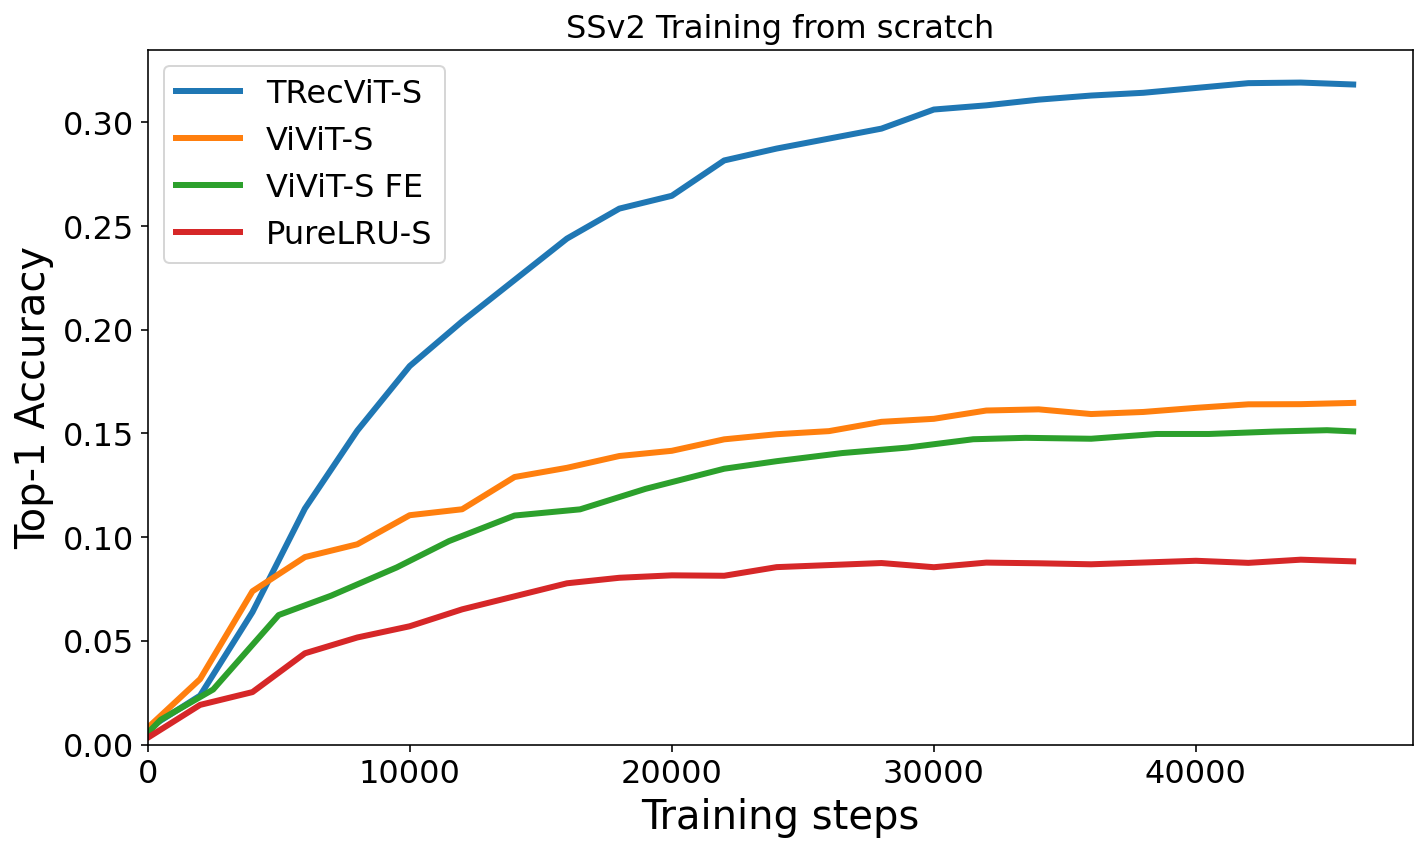
\includegraphics[width=.9\linewidth]{img/scratch.png}
  \caption{\ssm\ compared to baselines on supervised video classification on SSv2 dataset, trained from scratch. The plot shows the evolution of the evaluation accuracy as training progresses.
  }

  \label{fig:baselines}
\end{figure}
 

 \begin{figure*}[h]
  \centering
  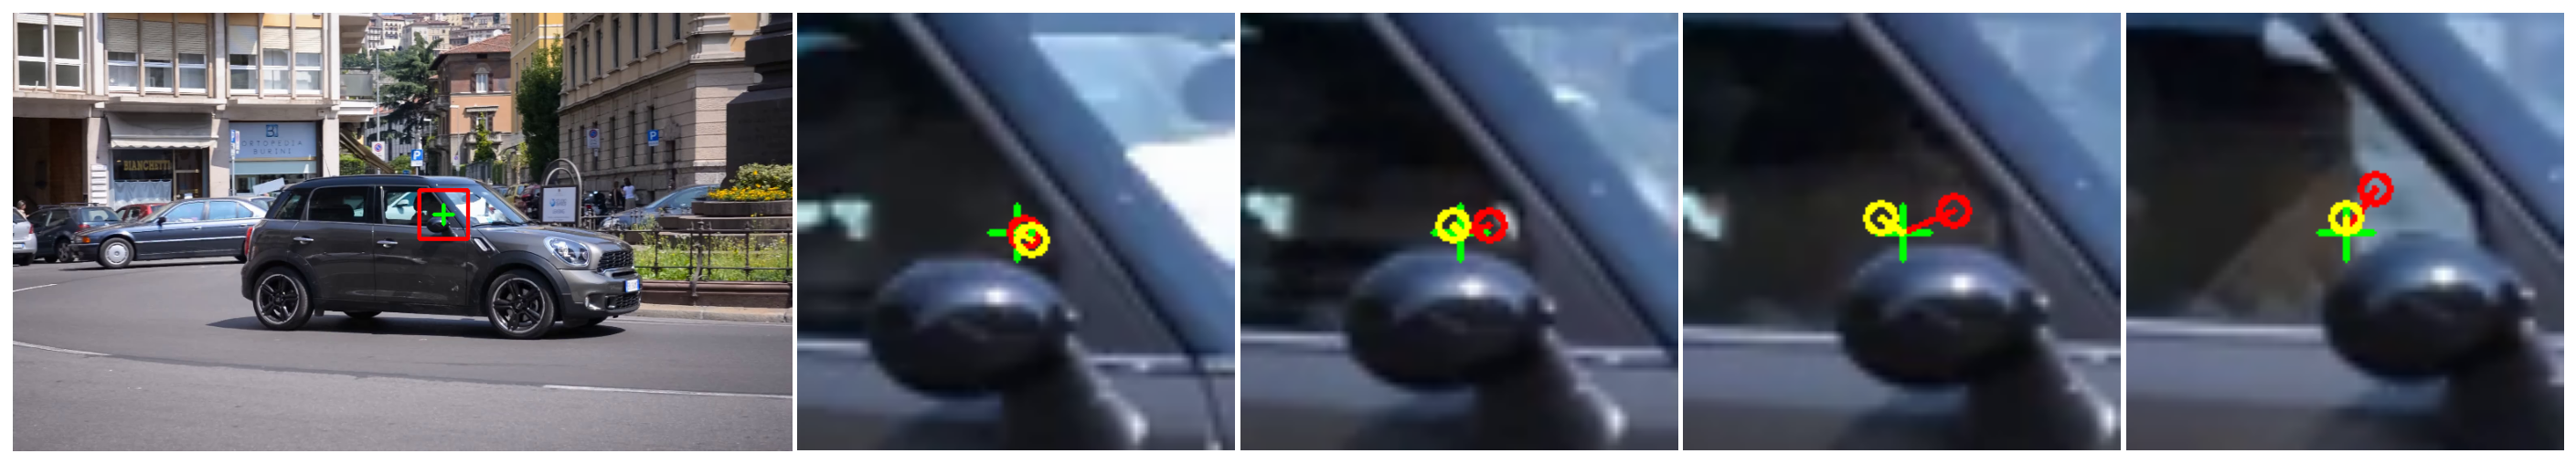
\includegraphics[width=\linewidth]{img/davis.png}
  \caption{Qualitative results obtained by \ssm\ for point tracking on DAVIS dataset compared to VideoMAE. The leftmost image indicates the point to track in the original frame, and the images towards the right show zoom-ins on subsequent frames. Green plus (+) marker indicates the ground truth, yellow circle indicates \ssm's predictions and red circles indicate VideoMAE's predictions.}
  \label{fig:tracking}
\end{figure*}


\begin{table}
    \centering
    \small{
    \begin{tabular}{l|c|c|r}
    \hline
    \textbf{Model} & \textbf{Patch size} & \textbf{Top-1 acc (\%)} & \textbf{\# params} \\
    \hline
    ViViT-B & (2, 16, 16) & 59.1 & 90M \\
    ViViT-L & (2, 16, 16) & 65.9 & 320M \\
    \ssm\ & (1, 16, 16) & \textbf{66.8} & 109M\\
    \hline
    \end{tabular}}
    \caption{Performance of \ssm\ compared to ViViT-B and ViViT-L baselines on SSv2 dataset with all models initialised from Imagenet pre-training. For ViViT-L, we use the result reported by its authors, for ViViT-B we obtained the results internally as they were not reported in the original paper for this dataset.}
    \label{tab:ssv2}
    \end{table}
    
\begin{table}
    \centering
    \small{
    \begin{tabular}{l|c|c|r}
    \hline
    \textbf{Model} & \textbf{Patch size} & \textbf{Top-1 acc (\%)} & \textbf{\# params} \\
    \hline
    ViViT-B & (2, 16, 16) & 78.1 & 90M \\
    ViViT-L & (2, 16, 16) & \textbf{78.7} & 320M \\
    \ssm\ & (1, 16, 16) & 78.4 & 109M\\
    \hline
    \end{tabular}}
    \caption{Performance of \ssm\ compared to ViViT-B and ViViT-L baselines on Kinetics400 dataset, with all models initialised from Imagenet pre-training. For ViViT-B and ViViT-L, we include the result we obtained internally by re-training the model on the current Kinetics400 dataset version; see footnote. In the original paper, the authors reported 80.3\% on Kinetics400 for ViViT-L.}
    \label{tab:kinetics}
    \end{table}

\subsection{Self-supervised masked autoencoding}
\label{sec:mae}
We use Kinetics400 for self-supervised pre-training from scratch and we report results on multiple downstream datasets and tasks by fine-tuning attention readout heads on top of frozen representations. We choose this setup, as opposed to fine-tuning end-to-end, as the  performance in this case more clearly reflects the quality of the pre-trained representations. As mentioned in the previous section, we use a large masking ratio (0.90), which makes pre-training very efficient. We report the number of parameters for every model considered. Note that the number of parameters for \ssm\ is different from the one reported in the previous section due to the addition of the readout heads.

\par \noindent \textbf{Video classification:}  We report video classification accuracy as downstream task using attention readout heads on SSv2 and Kinetics400. We compare the performance against VideoMAE-L~\cite{tong2022videomae} in Table~\ref{tab:selfsup}. Our model obtains slightly better performance on both datasets compared to this strong baseline, despite having almost 3$\times$ less parameters. 

\par \noindent \textbf{Point tracking:} To demonstrate that our model can handle dense(r) tasks as well, we evaluate the same frozen MAE representations for the point tracking task. We use the recurrent architecture in MooG~\cite{steenkiste2024moving} as a readout due to its simplicity. MooG uses light cross-attention layers to process the embeddings of each frame in order, and the readout state is carried over through time. We finetune the MooG readout head using MOVi-E dataset~\cite{movie} as done in popular point tracking works~\cite{DoerschYVG0ACZ23}. We evaluate these fine-tuned representations on two datasets: Perception Test~\citep{patraucean2023perception} and DAVIS dataset~\cite{davis2017} with point tracks extracted in~\cite{doersch2022tapvid}. We report average Jaccard metric~\cite{doersch2022tapvid} for \ssm\ compared with MooG and VideoMAE; see Table~\ref{tab:pt}. \ssm\ obtains better performance on both datasets compared to baselines, which reinforces the observation that our proposed model has strong motion modelling capabilities. We include qualitative results for this task in Figure~\ref{fig:tracking}. We can observe that the results are visibly better compared to VideoMAE. More visualisations are included in the supplementary material.

\begin{table}
    \centering
    \small{
    \begin{tabular}{l|c|c|r}
    \hline
    \textbf{Model} & \textbf{Dataset} & \textbf{Top-1 acc (\%)} & \textbf{\# params} \\
    \hline
    VideoMAE & Kinetics400 & 45.8 & 330M \\
    \ssm\ & Kinetics400 & \textbf{46.0} & 128M\\
    \hline
    \hline
    VideoMAE & SSv2 &  53.7 & 330M \\
    \ssm\ & SSv2 &  \textbf{53.9} & 128M\\
    \hline
    \end{tabular}}
    \caption{Performance of \ssm\ compared to VideoMAE on video classification using frozen MAE representations, pre-trained on Kinetics400.}
    \label{tab:selfsup}
    \end{table}

\begin{table}
    \centering
    \small{
    \begin{tabular}{l|c|c|c|r}
    \hline
    \textbf{Model} & \textbf{Dataset} & \textbf{\# frames} & \textbf{AJ} & \textbf{\# params} \\
    \hline
    MooG & DAVIS & 8 & 0.687 & 35M \\
    VideoMAE & DAVIS & 8 & 0.703 & 330M \\
    \ssm\ & DAVIS & 8 & \textbf{0.706} & 128M\\
    
    \hline
    \hline
    MooG & Perception Test & 16 & 0.760 & 46.5M \\
    VideoMAE & Perception Test & 16 & 0.761 & 330M \\
    \ssm\ & Perception Test & 16 & \textbf{0.783} & 128M\\
    \hline
    \end{tabular}}
    \caption{Performance of \ssm\ compared to baselines on point tracking task on DAVIS and Perception Test datasets. All models use frozen representations evaluated using the readout head from MooG.}
    \label{tab:pt}
    \end{table}

\begin{figure*}[h]
  \centering
  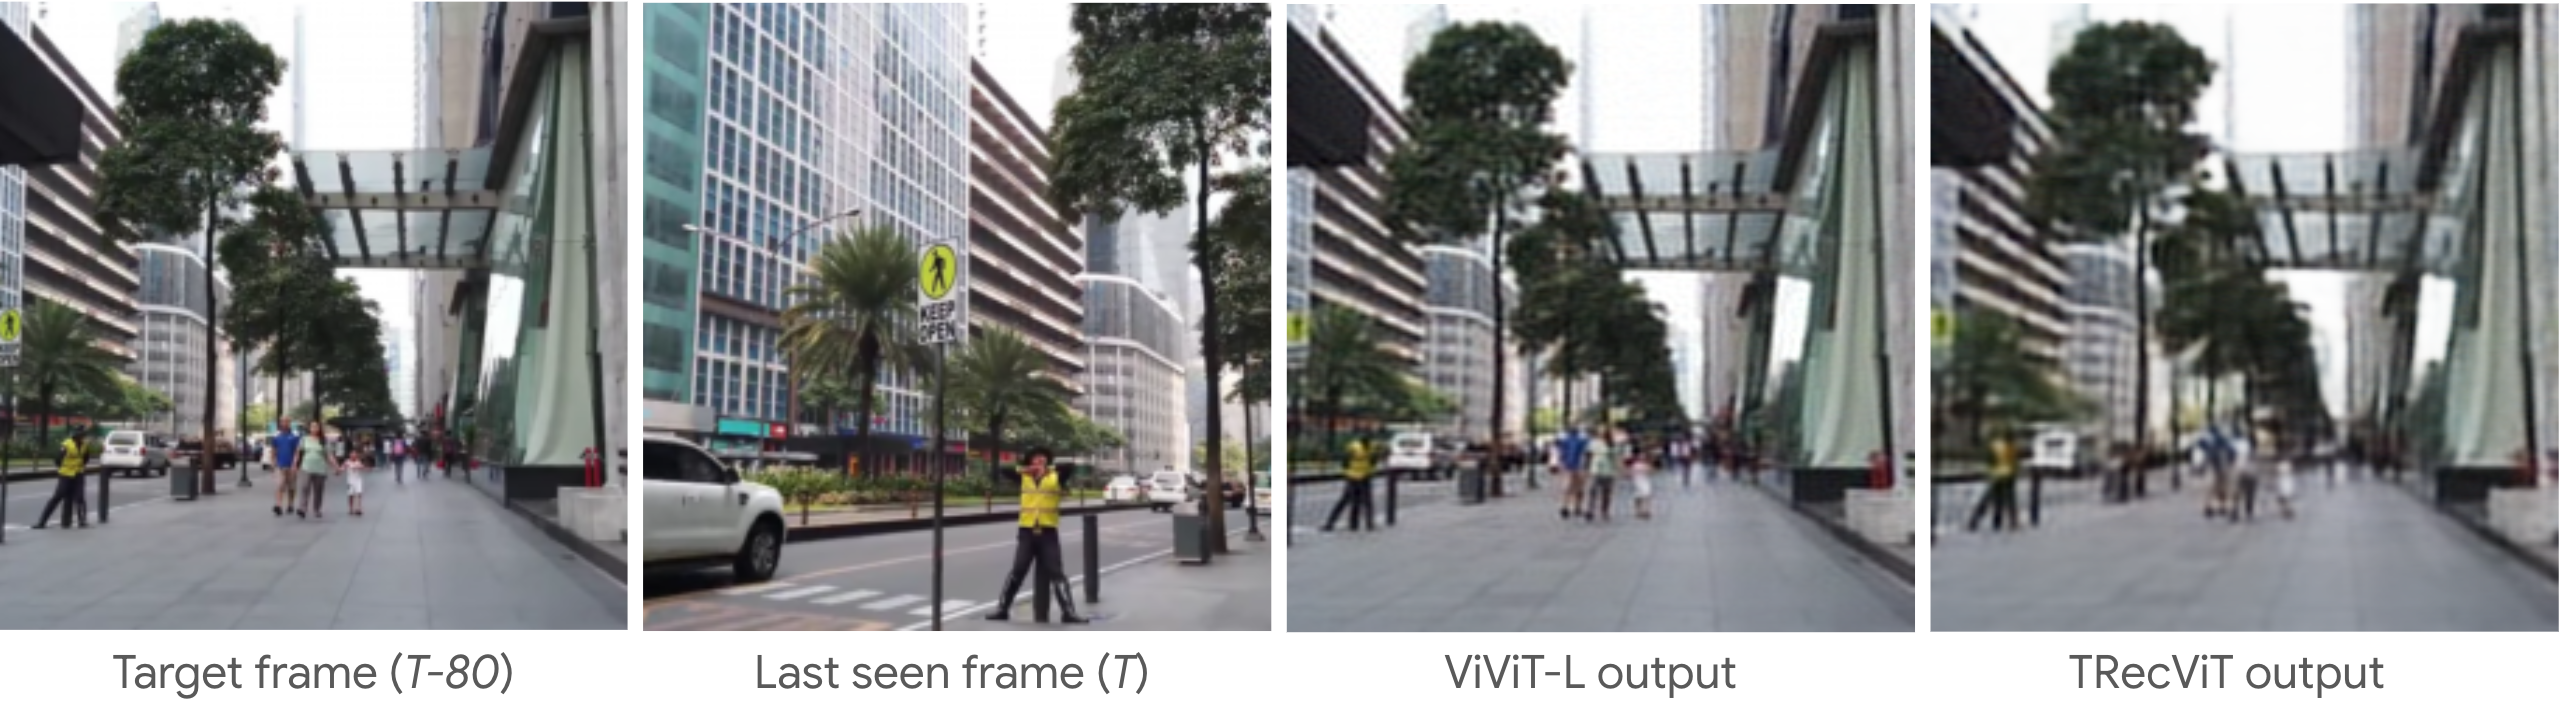
\includegraphics[width=\linewidth]{img/wtlong.png}
  \caption{Qualitative results obtained by \ssm\ on the dense memorisation task compared to ViViT-L. Both models are trained using Imagenet pre-trained weights, on video sequences of $T=64$ frames and they reconstruct the $(T-48)^\text{th}$ frame.}
  \label{fig:wt}
\end{figure*}

\begin{figure}[t]
\centering
\begin{subfigure}{0.48\linewidth}
    \centering
    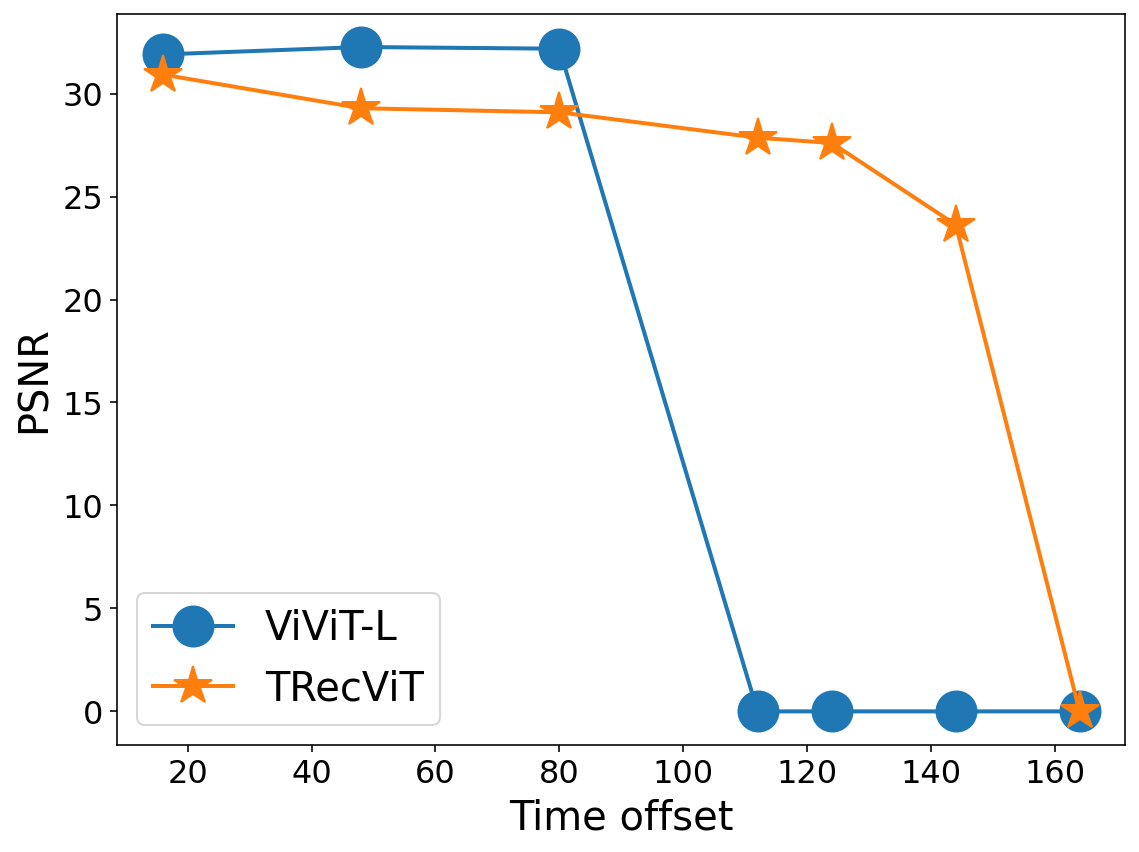
\includegraphics[width=\textwidth]{img/psnr.png}
    \caption{PSNR comparison}
\end{subfigure}%
\hfill
\begin{subfigure}{0.48\linewidth}
    \centering
    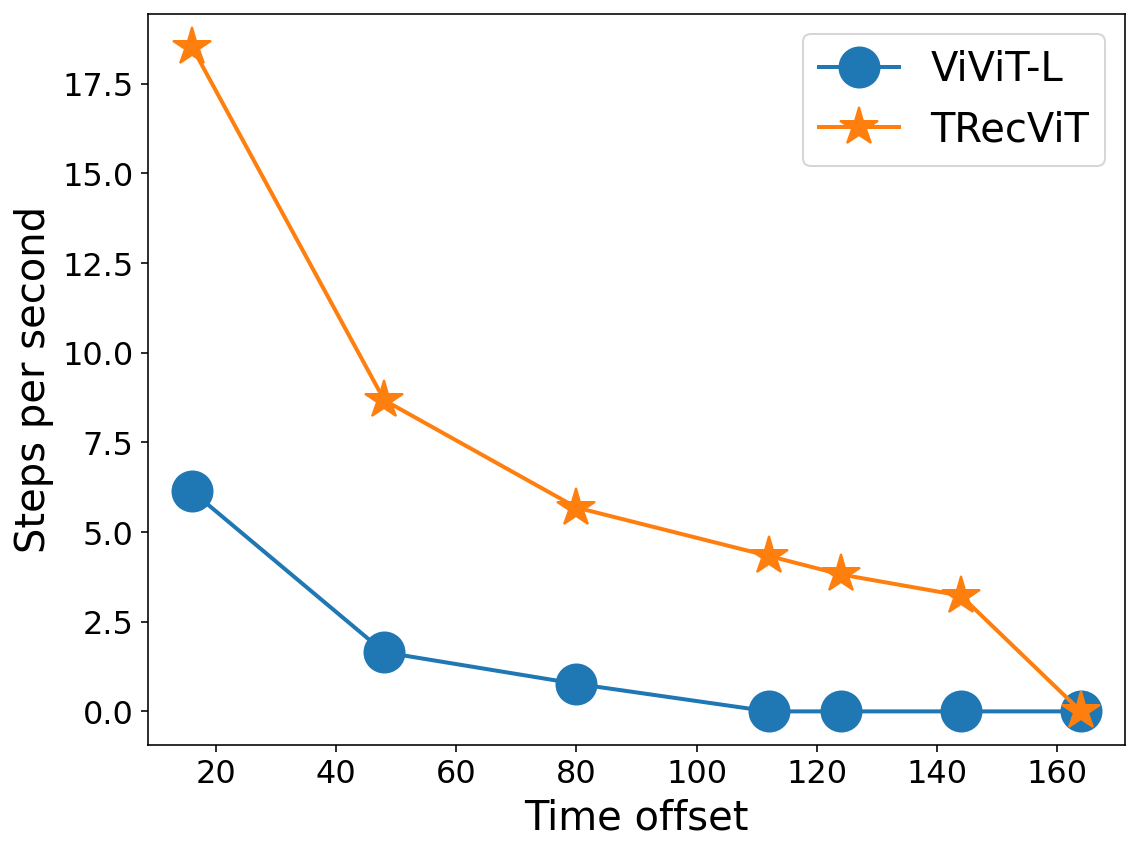
\includegraphics[width=\textwidth]{img/sps.png} 
    \caption{Steps-per-second comparison}
\end{subfigure}
\caption{Long video memorisation task. At time $T$, the model has to reconstruct the $(T-k)^\text{th}$ frame seen in the past. The plots show PSNR and throughput (steps-per-second) for increasing time offset $k$. For both models, the data points with $0$ value on the $y$-axis correspond to OOM.
}
\label{fig:psnr}
\end{figure}

\subsection{Long video memorisation task}
\label{sec:longtask}

Transformer models for language are known to be excellent at retrieving information from context, as they cache the keys and values for the entire history. On the other hand, LRUs / SSMs and RNNs in general struggle with such \emph{needle-in-the-haystack} style tasks as they need to perform the retrieval based on the compressed history kept in their recurrent state~\cite{jelassi2024repeat, de2024griffinmixinggatedlinear}. 
We are interested in studying this aspect in the video domain as well. We set up a simple reconstruction task where the model has to remember the frame seen at a given time-step in the past. For our analysis, we run multiple experiments where the model is tasked to reconstruct the $(T-k)^{\text{th}}$ frame from the past, with increasing value for $k\in\{16, 48, 80, 112, 144, 164\}$ frames. We employ Walking Tours dataset~\cite{venkataramanan2023imagenet}, which contains hour-long videos, and the scenery changes constantly, hence we are guaranteed that the video frames seen most recently will be very different compared to the frames seen earlier on. We scale the videos to $224\times224$ pixels. Again, we adopt ViViT-L as baseline, and we train both models using Imagenet pretrained weights. For ViViT-L, we keep all the outputs from all $T$ time steps and apply temporal pooling and a $1\times1$ convolution to get the expected shape for the reconstructed frame. For \ssm, we simply keep the output of the last layer at time step $T$ and reshape it to the expected shape. We show quantitative and qualitative results respectively in Figures~\ref{fig:psnr} and~\ref{fig:wt}. We can observe that there is a performance--efficiency trade-off at play for \ssm: its performance is slightly below ViViT's for shorter memory spans (16, 48, 80), but its efficiency (steps-per-second) is significantly higher. However, beyond 80 frames, ViViT-L goes out of memory, whilst \ssm\ continues to give decent results up to 144 frames, going out of memory towards 164 frames. Figure~\ref{fig:wt} shows qualitative results compared to the baseline for the case where the models have to remember the frame seen at $T-48$ in the past. We can observe that the quality of ViViT-L's reconstruction is good. For \ssm, whilst the overall structure (encoded in lower frequencies) is correct, it struggles to remember the high-frequency content of the image. This is to be expected due to the compression happening in the recurrent state of the model. However, given how different the last seen frame is from the target frame, we consider this to be a very promising result that warrants further investigation into the memorisation capabilities of our model, which we leave as future work.

\subsection{Generalisation to longer sequences}
\label{sec:gentask}

Using the same task as above, we analyse the generalisation capabilities to sequences longer than those used during training. Specifically, we train the models with sequences of length $T=64$ frames to reconstruct the $T-48$ frame, and evaluate them on longer sequences $T=96$ to reconstruct the same frame. The \ssm\ model can run on longer sequences without any modification. For the ViViT model, we need to adapt the positional encoding to accommodate longer sequences. We use interpolation to nearest neighbour to obtain the desired length; cubic interpolation led to worse results. The performance of \ssm\ degrades slightly, with PSNR going down from 29.3 (when evaluated on the same sequence length as in training $T=64$) to 26.4 when evaluated with $T=96$ frame sequences. ViViT's PSNR, however, drops significantly, from 32.3 when evaluated on the same sequence length, to 15.1 when evaluated on longer sequences. We include qualitative examples in Figure~\ref{fig:gentask} where we can observe that ViViT's output contains stronger artefacts compared to \ssm. 

\begin{figure}[h]
  \centering
  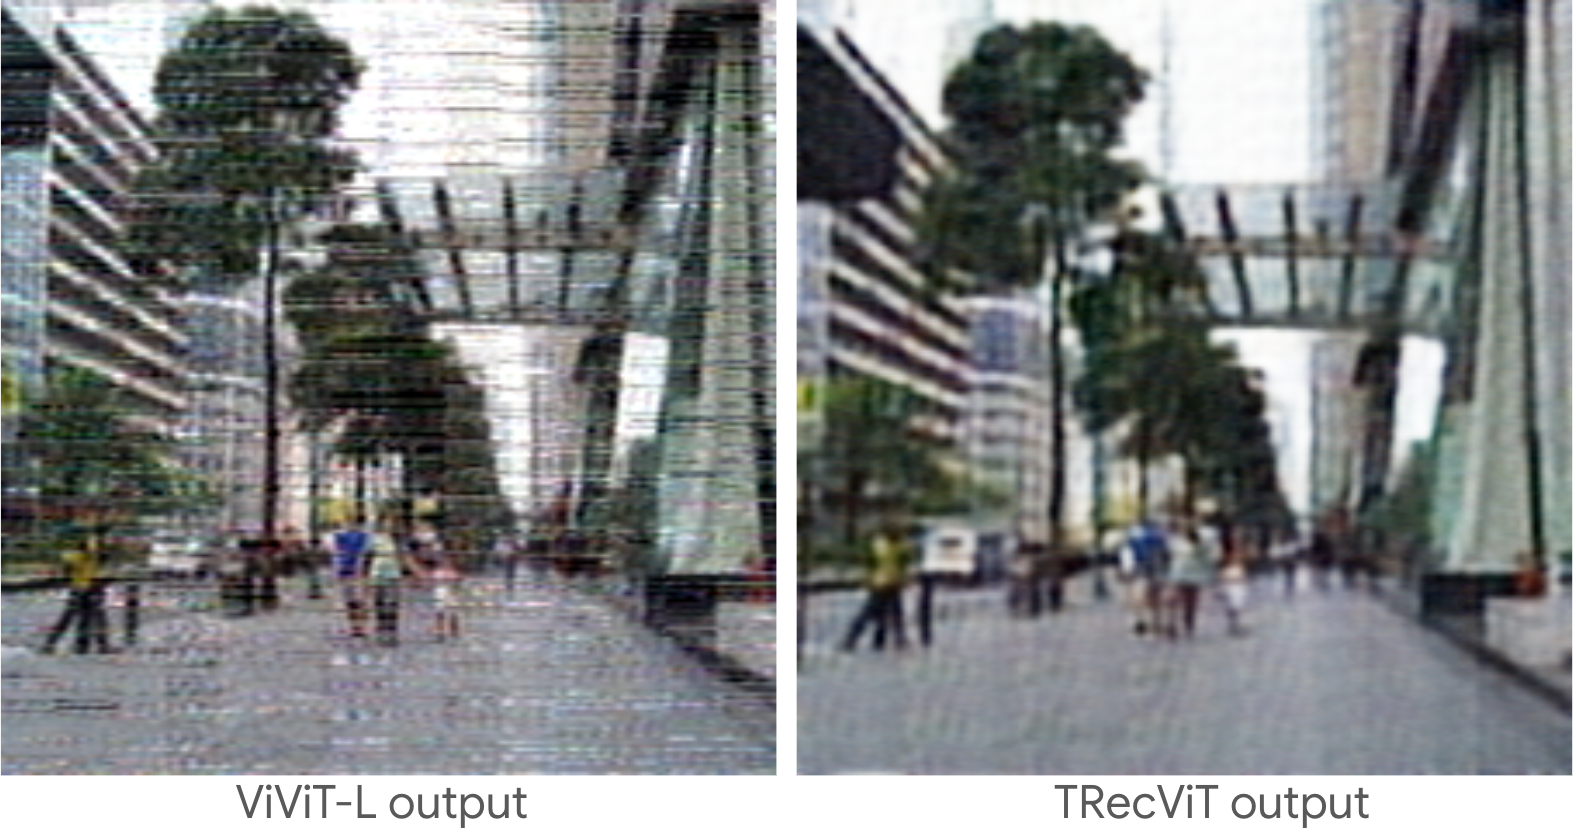
\includegraphics[width=\linewidth]{img/genlong.png}
  \caption{Generalisation to longer sequences. Both models are trained using Imagenet pre-trained weights, on video sequences of $T=64$ frames to reconstruct the $(T-48)^\text{th}$ frame; during evaluation, the models receive sequences of $T=96$ frames.}
  \label{fig:gentask}
\end{figure}

\section{Conclusion}
\label{sec:conclusion}
In this paper, we have investigated the common and unresolved issue that many established neural networks suffer from low floating-point operations per second (FLOPS). We have revisited a bottleneck operator, DWConv, and analyzed its main cause for a slowdown -- frequent memory access. To overcome the issue and achieve faster neural networks, we have proposed a simple yet fast and effective operator, PConv, that can be readily plugged into many existing networks. We have further introduced our general-purpose FasterNet, built upon our PConv, that achieves state-of-the-art speed and accuracy trade-off on various devices and vision tasks. We hope that our PConv and FasterNet would inspire more research on simple yet effective neural networks, going beyond academia to impact the industry and community directly.


\medskip\noindent\textbf{Acknowledgement} \enspace
This work was supported, in part, by Hong Kong General Research Fund under grant number 16200120. The work of C.-H. Lee was supported, in part, by the NSF under Grant IIS-2209921.
% \clearpage
\appendix
\addcontentsline{toc}{section}{Appendix}
\section*{\Large Appendix}
In this appendix, we provide further details on the experimental settings, full comparison plots, architectural configurations, PConv implementations, comparisons with related work, limitations, and future work.

\section{ImageNet-1k experimental settings}
\label{imagenet_settings}
We provide ImageNet-1k training and evaluation settings in~\cref{tab:imagenet_settings}. They can be used for reproducing our main results in~\cref{tab:imagenet} and \cref{fig:imageent}. Different FasterNet variants vary in the magnitude of regularization and augmentation techniques. The magnitude increases as the model becomes larger to alleviate overfitting and improve accuracy. Note that most of the compared works in~\cref{tab:imagenet} and \cref{fig:imageent}, \eg, MobileViT, EdgeNext, PVT, CycleMLP, ConvNeXt, Swin, \etc, also adopt such advanced training techniques (ADT). Some even heavily rely on the hyper-parameter search. For others w/o ADT, \ie, ShuffleNetV2, MobileNetV2, and GhostNet, though the comparison is not totally fair, we include them for reference.

\section{Downstream tasks experimental settings}
For object detection and instance segmentation on the COCO2017 dataset, we equip our FasterNet backbone with the popular Mask R-CNN detector. 
We use ImageNet-1k pre-trained weights to initialize the backbone and Xavier to initialize the add-on layers. Detailed settings are summarized in~\cref{tab:coco_settings}.

\section{Full comparison plots on ImageNet-1k}
\cref{fig:imagenet_full} shows the full comparison plots on ImageNet-1k, which is the extension of~\cref{fig:imageent} in the main paper with a larger range of latency. \cref{fig:imagenet_full} shows consistent results that FasterNet strikes better trade-offs than others in balancing accuracy and latency/throughput on GPU, CPU, and ARM processors.

\section{Detailed architectural configurations}
We present the detailed architectural configurations in~\cref{tab:configuration}. While different FasterNet variants share a unified architecture, they vary in the network width (the number of channels) and network depth (the number of FasterNet blocks at each stage). The classifier at the end of the architecture is used for classification tasks but removed for other downstream tasks. 


% Please add the following required packages to your document preamble:
% If you use beamer only pass "xcolor=table" option, i.e. \documentclass[xcolor=table]{beamer}
\begin{table}
\vspace{0.1in}
\centering
\resizebox{1\linewidth}{!}{%
\begin{tabular}{@{}l|cccccc@{}}
\toprule
Variants           & T0                         & T1    & T2    & S    & M     & L            \\ \midrule
Train Res          & \multicolumn{6}{c}{192 for epoch 1$\sim$280, 224 for epoch 281$\sim$300}                                    \\
Test Res           & \multicolumn{6}{c}{224}                                    \\ \midrule
Epochs             & \multicolumn{6}{c}{300}                                    \\
\# of forward pass & \multicolumn{6}{c}{188k}                                   \\ \midrule
Batch size         & 4096   & 4096      & 4096      & 4096      & 2048  & 2048\\
Optimizer          & \multicolumn{6}{c}{AdamW}                                  \\
Momentum & \multicolumn{6}{c}{0.9/0.999}                              \\
LR                 & 0.004  & 0.004 & 0.004 & 0.004 & 0.002 & 0.002             \\
LR decay           & \multicolumn{6}{c}{cosine}                                 \\
Weight decay       & 0.005  & 0.01  & 0.02  & 0.03  & 0.05 & 0.05               \\
Warmup epochs      & \multicolumn{6}{c}{20}                                     \\
Warmup schedule    & \multicolumn{6}{c}{linear}                                 \\ \midrule
Label smoothing    & \multicolumn{6}{c}{0.1}                                    \\
Dropout            & \multicolumn{6}{c}{{\color[HTML]{9B9B9B} \ding{55}}}       \\
Stoch. Depth       & {\color[HTML]{9B9B9B} \ding{55}}   & 0.02  & 0.05  & 0.1  & 0.2  & 0.3   \\
Repeated Aug       & \multicolumn{6}{c}{{\color[HTML]{9B9B9B} \ding{55}}}       \\
Gradient Clip.     & {\color[HTML]{9B9B9B} \ding{55}}   & {\color[HTML]{9B9B9B} \ding{55}}  & {\color[HTML]{9B9B9B} \ding{55}}  & {\color[HTML]{9B9B9B} \ding{55}}  & 1  & 0.01       \\ \midrule
% Gradient Clip.     & \multicolumn{6}{c}{{\color[HTML]{9B9B9B} \ding{55}}}       \\ \midrule
H. flip            & \multicolumn{6}{c}{\ding{51}}                              \\
RRC                & \multicolumn{6}{c}{\ding{51}}                              \\
Rand Augment       & {\color[HTML]{9B9B9B} \ding{55}}   & 3/0.5 & 5/0.5 & 7/0.5 & 7/0.5 & 7/0.5 \\
Auto Augment       & \multicolumn{6}{c}{{\color[HTML]{9B9B9B} \ding{55}}}       \\
Mixup alpha        & 0.05                        & 0.1   & 0.1   & 0.3   & 0.5   & 0.7           \\
Cutmix alpha       & \multicolumn{6}{c}{1.0}                                    \\
Erasing prob. & \multicolumn{6}{c}{{\color[HTML]{9B9B9B} \ding{55}}} \\
Color Jitter       & \multicolumn{6}{c}{{\color[HTML]{9B9B9B} \ding{55}}}       \\
PCA lighting       & \multicolumn{6}{c}{{\color[HTML]{9B9B9B} \ding{55}}}       \\ \midrule
SWA                & \multicolumn{6}{c}{{\color[HTML]{9B9B9B} \ding{55}}}       \\
EMA                & \multicolumn{6}{c}{{\color[HTML]{9B9B9B} \ding{55}}}       \\ \midrule
Layer scale    & \multicolumn{6}{c}{{\color[HTML]{9B9B9B} \ding{55}}}                          \\ \midrule
CE loss            & \multicolumn{6}{c}{\ding{51}}                              \\
BCE loss           & \multicolumn{6}{c}{{\color[HTML]{9B9B9B} \ding{55}}}       \\ \midrule
Mixed precision    & \multicolumn{6}{c}{\ding{51}}                              \\ \midrule
Test crop ratio        & \multicolumn{6}{c}{0.9}       \\ \midrule
Top-1 acc. (\%)         & 71.9   & 76.2 & 78.9  & 81.3  & 83.0  &   83.5    \\ \bottomrule
\end{tabular}%
}
\caption{ImageNet-1k training and evaluation settings for different FasterNet variants.}
\label{tab:imagenet_settings}
\end{table}
% Please add the following required packages to your document preamble:
% \usepackage{booktabs}
% \usepackage{graphicx}
\begin{table}
\centering
\vspace{0.2in}
\resizebox{\linewidth}{!}{%
\setlength{\tabcolsep}{6pt}
\begin{tabular}{@{}l|ccc@{}}
\toprule
Variants & \qquad S \qquad \qquad           & \qquad M \qquad \qquad      & L\\ \midrule
Train and test Res & \multicolumn{3}{c}{shorter side $=$ 800, longer side $\leq$ 1333} \\
Batch size                    & \multicolumn{3}{c}{16 (2 on each GPU)} \\
Optimizer                     & \multicolumn{3}{c}{AdamW}              \\
Train schedule     & \multicolumn{3}{c}{1$\times$ schedule (12 epochs)}                      \\
Weight decay                  & \multicolumn{3}{c}{0.0001}             \\
Warmup schedule               & \multicolumn{3}{c}{linear}             \\
Warmup iterations             & \multicolumn{3}{c}{500}                \\
LR decay           & \multicolumn{3}{c}{StepLR at epoch 8 and 11 with decay rate 0.1}             \\
LR                            & 0.0002      & 0.0001      & 0.0001     \\
Stoch. Depth                  & 0.15        & 0.2         & 0.3        \\ \bottomrule
\end{tabular}%
}
\caption{Experimental settings of object detection and instance segmentation on the COCO2017 dataset.}
\vspace{-0.2in}
\label{tab:coco_settings}
\end{table}
\begin{figure*}
    \centering
    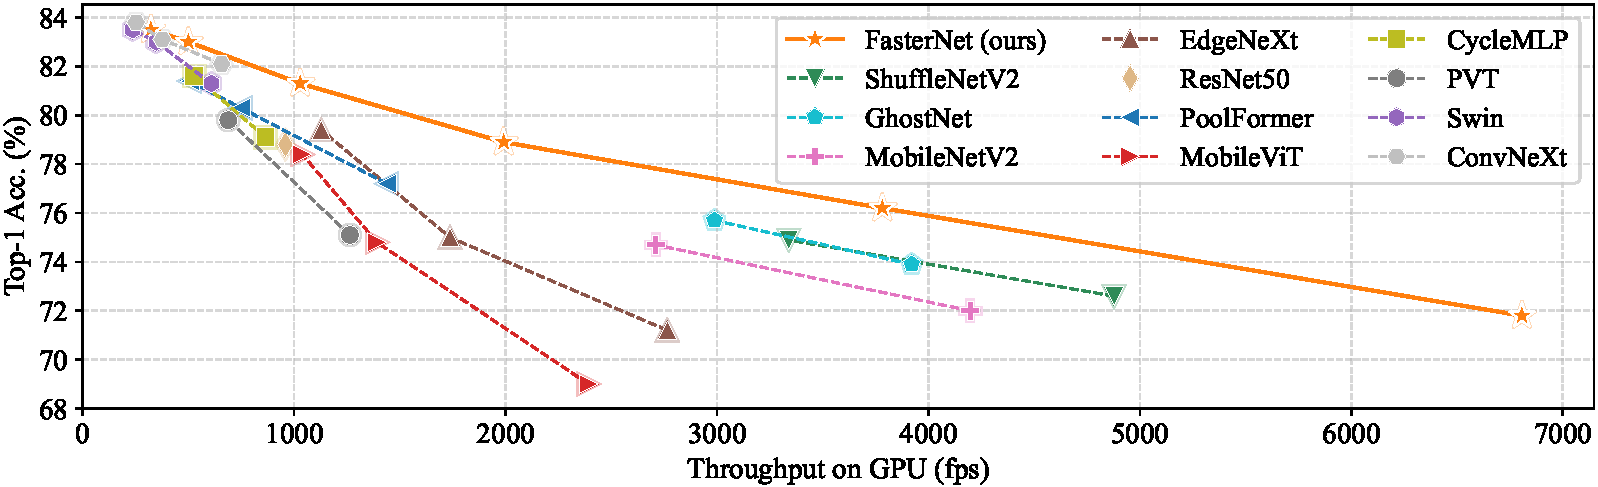
\includegraphics[width=1.\linewidth]{figures/fps_latency_gpu-cropped.pdf}

    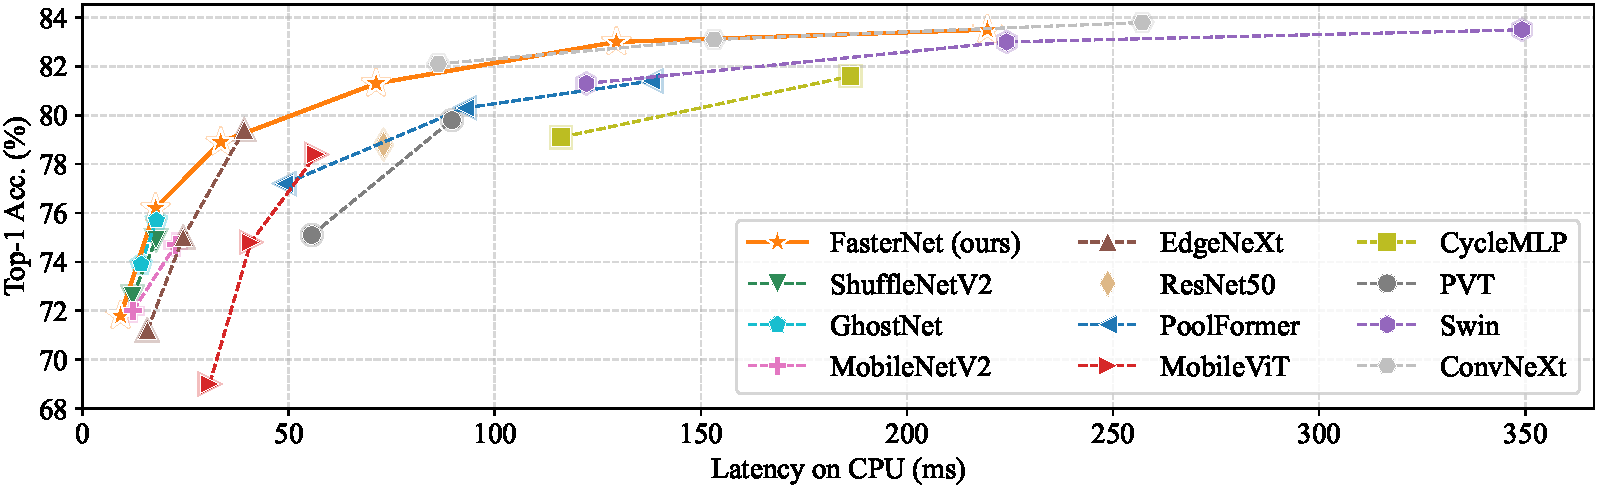
\includegraphics[width=1.\linewidth]{figures/acc_latency_cpu-cropped.pdf}
    
    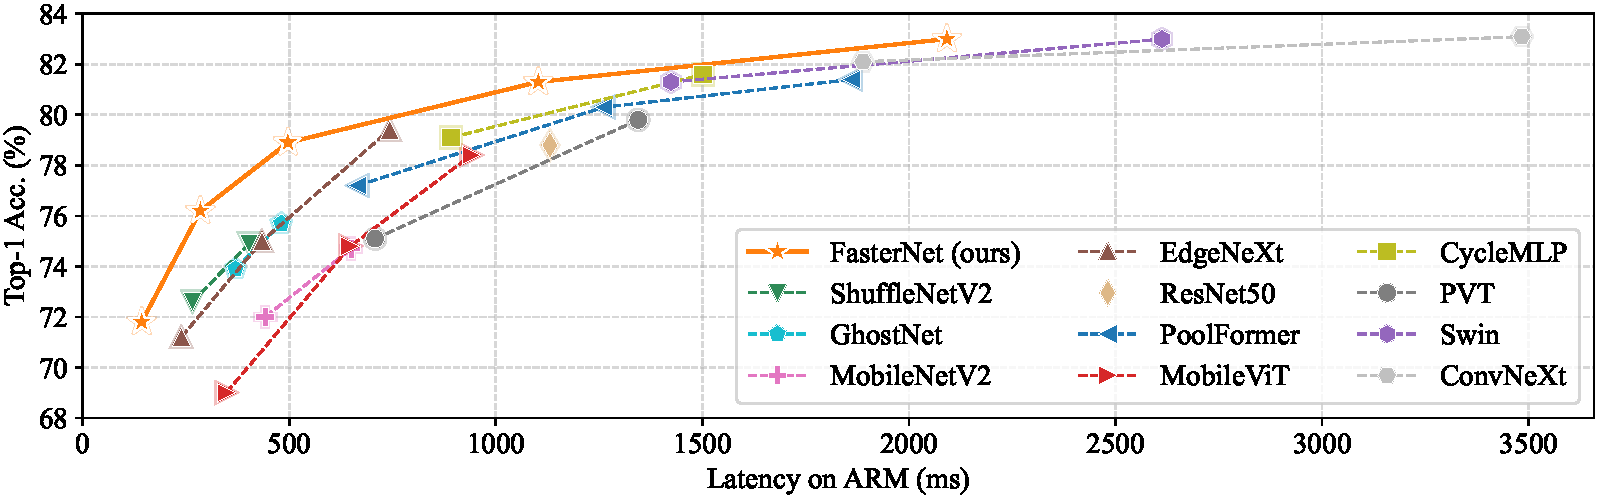
\includegraphics[width=1.\linewidth]{figures/acc_latency_arm-cropped.pdf}
    
    \vspace{-0.1in}
    \caption{Comparison of FasterNet with state-of-the-art networks. FasterNet consistently achieves better accuracy-throughput (the top plot) and accuracy-latency (the medium and bottom plots) trade-offs than others.}
    \label{fig:imagenet_full}
\end{figure*}

% \section{Implementation of PConv}
% We provide the PyTorch-based implementation of PConv in~\cref{lst:code}. There are two forward pass choices, namely forward\_slicing and forward\_split\_cat. The forward\_slicing choice writes the convolutional output in place of the input, which is used for faster inference, but not for training, as the in-place operation modifies the gradient computation. By contrast, the forward\_split\_cat choice concatenates the convolutional output with the feature maps untouched, which preserves the intermediate gradient computation and is used for training. \cref{tab:pconv_implementation} shows the speed comparison of these two choices during inference. The forward\_slicing implementation runs faster than the other one, especially for tiny models and more computation-powerful devices, \eg, for FasterNet-T0 on GPU.

\section{More comparisons with related work}
\medskip\noindent\textbf{Improving FLOPS.} \enspace 
There are a few other works~\cite{ding2022scaling_short,xia2022trt_short} also looking into the FLOPS issue and trying to improve it. They generally follow existing operators and try to find their proper configurations, \eg, RepLKNet~\cite{ding2022scaling_short} simply increases the kernel size while TRT-ViT~\cite{xia2022trt_short} reorders different blocks in the architecture. By contrast, this paper advances the field by proposing a novel and efficient PConv, opening up new directions and potentially larger room for FLOPS improvement.

% \clearpage
% Please add the following required packages to your document preamble:
% \usepackage{booktabs}
% \usepackage{graphicx}
\begin{table*}
\centering
\resizebox{.93\linewidth}{!}{%
% \setlength{\tabcolsep}{1pt}
\begin{tabular}{@{}c|c|c|c|c|c|c|c|c|c@{}}
\toprule
Name &
  Output size &
  \multicolumn{2}{c|}{Layer specification} &
  T0 &
  T1 &
  T2 &
  S &
  M &
  L \\ \midrule
Embedding &
  \large{$\frac{h}{4} \times \frac{w}{4}$}&
  \begin{tabular}[c]{@{}c@{}}Conv\_4\_$c$\_4,\\ BN\end{tabular} &
  \# Channels $c$ &
  40 &
  64 &
  96 &
  128 &
  144 &
  192 \\ \midrule
Stage 1 &
  \large{$\frac{h}{4} \times \frac{w}{4}$}&
  $\left[ \text{\begin{tabular}[c]{@{}c@{}}PConv\_3\_$c$\_1\_1/4,\\ Conv\_1\_$2c$\_1,\\ BN, Acti,\\ Conv\_1\_$c$\_1\end{tabular}}  \right] \times b_1 $  &
  \# Blocks $b_1$ &
  1 &
  1 &
  1 &
  1 &
  3 &
  3 \\ \midrule
Merging &
  \large{$\frac{h}{8} \times \frac{w}{8}$}&
  \begin{tabular}[c]{@{}c@{}}Conv\_2\_$2c$\_2,\\ BN\end{tabular} &
  \# Channels $2c$ &
  80 &
  128 &
  192 &
  256 &
  288 &
  384 \\ \midrule
Stage 2 &
  \large{$\frac{h}{8} \times \frac{w}{8}$}&
  $\left[ \text{\begin{tabular}[c]{@{}c@{}}PConv\_3\_$2c$\_1\_1/4,\\ Conv\_1\_$4c$\_1,\\ BN, Acti,\\ Conv\_1\_$2c$\_1\end{tabular}}  \right] \times b_2 $  &
  \# Blocks $b_2$ &
  2 &
  2 &
  2 &
  2 &
  4 &
  4 \\ \midrule
Merging &
  \large{$\frac{h}{16} \times \frac{w}{16}$}&
  \begin{tabular}[c]{@{}c@{}}Conv\_2\_$4c$\_2,\\ BN\end{tabular} &
  \# Channels $4c$ &
  160 &
  256 &
  384 &
  512 &
  576 &
  768 \\ \midrule
Stage 3 &
  \large{$\frac{h}{16} \times \frac{w}{16}$}&
  $\left[ \text{\begin{tabular}[c]{@{}c@{}}PConv\_3\_$4c$\_1\_1/4,\\ Conv\_1\_$8c$\_1,\\ BN, Acti,\\ Conv\_1\_$4c$\_1\end{tabular}}  \right] \times b_3 $  &
  \# Blocks $b_3$ &
  8 &
  8 &
  8 &
  13 &
  18 &
  18 \\ \midrule
Merging &
  \large{$\frac{h}{32} \times \frac{w}{32}$}&
  \begin{tabular}[c]{@{}c@{}}Conv\_2\_$8c$\_2,\\ BN\end{tabular} &
  \# Channels $8c$ &
  320 &
  512 &
  768 &
  1024 &
  1152 &
  1536 \\ \midrule
Stage 4 &
  \large{$\frac{h}{32} \times \frac{w}{32}$}&
  $\left[ \text{\begin{tabular}[c]{@{}c@{}}PConv\_3\_$8c$\_1\_1/4,\\ Conv\_1\_$16c$\_1,\\ BN, Acti,\\ Conv\_1\_$8c$\_1\end{tabular}}  \right] \times b_4 $  &
  \# Blocks $b_4$ &
  2 &
  2 &
  2 &
  2 &
  3 &
  3 \\ \midrule
Classifier &
  $1  \times 1$ &
  \begin{tabular}[c]{@{}c@{}}Global average pool,\\ Conv\_1\_1280\_1,\\ Acti,\\ FC\_1000\end{tabular} &
  Acti &
  GELU &
  GELU &
  ReLU &
  ReLU &
  ReLU &
  ReLU \\ \midrule
\multicolumn{4}{c|}{FLOPs (G)} &
  0.34 &
  0.85 &
  1.90 &
  4.55 &
  8.72 &
  15.49 \\ \midrule
\multicolumn{4}{c|}{Params (M)} &
  3.9 &
  7.6 &
  15.0 &
  31.1 &
  53.5 &
  93.4 \\ \bottomrule
\end{tabular}%
}
\caption{Configurations of different FasterNet variants. ``Conv\_$k$\_$c$\_$s$'' means a convolutional layer with the kernel size of $k$, the output channels of $c$, and the stride of $s$. ``PConv$\_k\_c\_s\_r$'' means a partial convolution with an extra parameter, the partial ratio of $r$. ``FC\_1000'' means a fully connected layer with 1000 output channels. $h \times w$ is the input size while $b_i$ is the number of FasterNet blocks at stage $i$. The FLOPs are calculated given the input size of $224 \times 224$.}
\label{tab:configuration}
\end{table*}
% \input{tables/pconv_implementation.tex}
% \input{tables/pconv_code.tex}
% \clearpage

\medskip\noindent\textbf{PConv vs. GConv.} \enspace 
PConv is schematically equivalent to a modified GConv~\cite{krizhevsky2012imagenet} that operates on a single group and leaves other groups untouched. Though simple, such a modification remains unexplored before. It's also significant in the sense that it prevents the operator from excessive memory access and is computationally more efficient. From the perspective of low-rank approximations, PConv improves GConv by further reducing the intra-filter redundancy beyond the inter-filter redundancy~\cite{haase2020rethinking_short}.

\medskip\noindent\textbf{FasterNet vs. ConvNeXt.} \enspace 
Our FasterNet appears similar to ConvNeXt~\cite{liu2022convnet} after substituting DWConv with our PConv. However, they are different in motivations. While ConvNeXt searches for a better structure by trial and error, we append PWConv after PConv to better aggregate information from all channels. Moreover, ConvNeXt follows ViT to use fewer activation functions, while we intentionally remove them from the middle of PConv and PWConv, to minimize their error in approximating a regular Conv. 

\medskip\noindent\textbf{Other paradigms for efficient inference.} \enspace 
Our work focuses on efficient network design, orthogonal to the other paradigms, \eg, neural architecture search (NAS)~\cite{elsken2019neural}, network pruning~\cite{molchanov2016pruning}, and knowledge distillation~\cite{hinton2015distilling}. They can be applied in this paper for better performance. However, we opt not to do so to keep our core idea centered and to make the performance gain clear and fair.

\medskip\noindent\textbf{Other partial/masked convolution works.} \enspace 
There are several works~\cite{liu2018image,gao2022convmae,liu2022partial} sharing similar names with our PConv. However, they differ a lot in objectives and methods. For example, they apply filters on partial pixels to exclude invalid patches~\cite{liu2018image}, enable self-supervised learning~\cite{gao2022convmae}, or synthesize novel images~\cite{liu2022partial}, while we target at the channel dimension for efficient inference. 

\section{Limitations and future work}
We have demonstrated that PConv and FasterNet are fast and effective, being competitive with existing operators and networks. Yet there are some minor technical limitations of this paper. For one thing, PConv is designed to apply a regular convolution on only a part of the input channels while leaving the remaining ones untouched. Thus, the stride of the partial convolution should always be 1, in order to align the spatial resolution of the convolutional output and that of the untouched channels. Note that it is still feasible to down-sample the spatial resolution as there can be additional downsampling layers in the architecture. 
And for another, our FasterNet is simply built upon convolutional operators with a possibly limited receptive field. Future efforts can be made to enlarge its receptive field and combine it with other operators to pursue higher accuracy.





% % Please add the following required packages to your document preamble:
% \usepackage{booktabs}
% \usepackage{graphicx}
\begin{table*}
\centering
\resizebox{.93\linewidth}{!}{%
% \setlength{\tabcolsep}{1pt}
\begin{tabular}{@{}c|c|c|c|c|c|c|c|c|c@{}}
\toprule
Name &
  Output size &
  \multicolumn{2}{c|}{Layer specification} &
  T0 &
  T1 &
  T2 &
  S &
  M &
  L \\ \midrule
Embedding &
  \large{$\frac{h}{4} \times \frac{w}{4}$}&
  \begin{tabular}[c]{@{}c@{}}Conv\_4\_$c$\_4,\\ BN\end{tabular} &
  \# Channels $c$ &
  40 &
  64 &
  96 &
  128 &
  144 &
  192 \\ \midrule
Stage 1 &
  \large{$\frac{h}{4} \times \frac{w}{4}$}&
  $\left[ \text{\begin{tabular}[c]{@{}c@{}}PConv\_3\_$c$\_1\_1/4,\\ Conv\_1\_$2c$\_1,\\ BN, Acti,\\ Conv\_1\_$c$\_1\end{tabular}}  \right] \times b_1 $  &
  \# Blocks $b_1$ &
  1 &
  1 &
  1 &
  1 &
  3 &
  3 \\ \midrule
Merging &
  \large{$\frac{h}{8} \times \frac{w}{8}$}&
  \begin{tabular}[c]{@{}c@{}}Conv\_2\_$2c$\_2,\\ BN\end{tabular} &
  \# Channels $2c$ &
  80 &
  128 &
  192 &
  256 &
  288 &
  384 \\ \midrule
Stage 2 &
  \large{$\frac{h}{8} \times \frac{w}{8}$}&
  $\left[ \text{\begin{tabular}[c]{@{}c@{}}PConv\_3\_$2c$\_1\_1/4,\\ Conv\_1\_$4c$\_1,\\ BN, Acti,\\ Conv\_1\_$2c$\_1\end{tabular}}  \right] \times b_2 $  &
  \# Blocks $b_2$ &
  2 &
  2 &
  2 &
  2 &
  4 &
  4 \\ \midrule
Merging &
  \large{$\frac{h}{16} \times \frac{w}{16}$}&
  \begin{tabular}[c]{@{}c@{}}Conv\_2\_$4c$\_2,\\ BN\end{tabular} &
  \# Channels $4c$ &
  160 &
  256 &
  384 &
  512 &
  576 &
  768 \\ \midrule
Stage 3 &
  \large{$\frac{h}{16} \times \frac{w}{16}$}&
  $\left[ \text{\begin{tabular}[c]{@{}c@{}}PConv\_3\_$4c$\_1\_1/4,\\ Conv\_1\_$8c$\_1,\\ BN, Acti,\\ Conv\_1\_$4c$\_1\end{tabular}}  \right] \times b_3 $  &
  \# Blocks $b_3$ &
  8 &
  8 &
  8 &
  13 &
  18 &
  18 \\ \midrule
Merging &
  \large{$\frac{h}{32} \times \frac{w}{32}$}&
  \begin{tabular}[c]{@{}c@{}}Conv\_2\_$8c$\_2,\\ BN\end{tabular} &
  \# Channels $8c$ &
  320 &
  512 &
  768 &
  1024 &
  1152 &
  1536 \\ \midrule
Stage 4 &
  \large{$\frac{h}{32} \times \frac{w}{32}$}&
  $\left[ \text{\begin{tabular}[c]{@{}c@{}}PConv\_3\_$8c$\_1\_1/4,\\ Conv\_1\_$16c$\_1,\\ BN, Acti,\\ Conv\_1\_$8c$\_1\end{tabular}}  \right] \times b_4 $  &
  \# Blocks $b_4$ &
  2 &
  2 &
  2 &
  2 &
  3 &
  3 \\ \midrule
Classifier &
  $1  \times 1$ &
  \begin{tabular}[c]{@{}c@{}}Global average pool,\\ Conv\_1\_1280\_1,\\ Acti,\\ FC\_1000\end{tabular} &
  Acti &
  GELU &
  GELU &
  ReLU &
  ReLU &
  ReLU &
  ReLU \\ \midrule
\multicolumn{4}{c|}{FLOPs (G)} &
  0.34 &
  0.85 &
  1.90 &
  4.55 &
  8.72 &
  15.49 \\ \midrule
\multicolumn{4}{c|}{Params (M)} &
  3.9 &
  7.6 &
  15.0 &
  31.1 &
  53.5 &
  93.4 \\ \bottomrule
\end{tabular}%
}
\caption{Configurations of different FasterNet variants. ``Conv\_$k$\_$c$\_$s$'' means a convolutional layer with the kernel size of $k$, the output channels of $c$, and the stride of $s$. ``PConv$\_k\_c\_s\_r$'' means a partial convolution with an extra parameter, the partial ratio of $r$. ``FC\_1000'' means a fully connected layer with 1000 output channels. $h \times w$ is the input size while $b_i$ is the number of FasterNet blocks at stage $i$. The FLOPs are calculated given the input size of $224 \times 224$.}
\label{tab:configuration}
\end{table*}
% \input{tables/pconv_implementation.tex}
% \clearpage
% \input{tables/pconv_code.tex}

%%%%%%%%% REFERENCES
{\small
\bibliographystyle{ieee_fullname}
\bibliography{egbib}
}

\end{document}
